%% ----------------------------------------------------------------------------------------
%% Author: Rajesh Siraskar
%% Date: 20-Jul-2023
%% An empirical study -- REINFORCE w.r.t. A2C, DQN and PPO
%% Build options: PdfLaTex + BibTex
%%
%% ----------------------------------------------------------------------------------------
\documentclass[a4paper, 12pt]{article}
\usepackage[T1]{fontenc}
\usepackage[utf8]{inputenc}
%\usepackage[round]{natbib} % Sort in order of occurence
\usepackage[round, authoryear, sort]{natbib}

\usepackage[pass]{geometry}
\usepackage{graphicx}
\graphicspath{{./images/}} % Images folder

%\usepackage{csquotes} 	% Quotes
\usepackage{listings}
\usepackage[table]{xcolor} %

\definecolor{codegreen}{rgb}{0,0.6,0}
\definecolor{codegray}{rgb}{0.5,0.5,0.5}
\definecolor{codepurple}{rgb}{0.58,0,0.82}
\definecolor{backcolour}{rgb}{0.95,0.95,0.92}

\lstdefinestyle{mystyle}{
	backgroundcolor=\color{backcolour},   
	commentstyle=\color{codegreen},
	keywordstyle=\color{magenta},
	numberstyle=\tiny\color{codegray},
	stringstyle=\color{codepurple},
	basicstyle=\ttfamily\footnotesize,
	breakatwhitespace=false,         
	breaklines=true,                 
	captionpos=b,                    
	keepspaces=true,                 
	numbers=left,                    
	numbersep=5pt,                  
	showspaces=false,                
	showstringspaces=false,
	showtabs=false,                  
	tabsize=2
}
\lstset{style=mystyle}

\usepackage{booktabs}	% Tables
\usepackage{arydshln} 	% dashed lines in tables
\usepackage{pdflscape}	% Landscape page
\usepackage{caption}
\usepackage{multirow}

\usepackage{subcaption}
\usepackage{amsfonts}
\usepackage{amsmath,amssymb}
\usepackage{textcomp}	% for \texttrademark
\usepackage{setspace}
\usepackage[spaces, hyphens]{url}
\usepackage[colorlinks, allcolors=blue]{hyperref}

% Macros
\newcolumntype{L}[1]{>{\raggedright\let\newline\\\arraybackslash\hspace{0pt}}m{#1}}
\newcolumntype{C}[1]{>{\centering\let\newline\\\arraybackslash\hspace{0pt}}m{#1}}
\newcolumntype{R}[1]{>{\raggedleft\let\newline\\\arraybackslash\hspace{0pt}}m{#1}}
\newcommand{\rowspace}[1]{\renewcommand{\arraystretch}{#1}}

\renewenvironment{abstract}
{\small
	\begin{center}
		\bfseries \abstractname\vspace{-.5em}\vspace{0pt}
	\end{center}
	\list{}{
		\setlength{\leftmargin}{.25cm}%
		\setlength{\rightmargin}{\leftmargin}%
	}%
	\item\relax}
{\endlist}

%% Quotes with epigraph style
\usepackage{epigraph}
% \epigraphsize{\small}% Default
\setlength\epigraphwidth{12cm}
\setlength\epigraphrule{0pt}
\usepackage{etoolbox}
\makeatletter
\patchcmd{\epigraph}{\@epitext{#1}}{\itshape\@epitext{#1}}{}{}
\makeatother
%% End Quotes macro

\title{An empirical study of the na\"ive REINFORCE algorithm for predictive maintenance of industrial milling machines}
\author{Rajesh Siraskar}

%% Squeezing space
\onehalfspacing
\renewcommand\floatpagefraction{.9}
\renewcommand\topfraction{.9}
\renewcommand\bottomfraction{.9}
\renewcommand\textfraction{.1}   
\setcounter{totalnumber}{50}
\setcounter{topnumber}{50}
\setcounter{bottomnumber}{50}

\begin{document}
\maketitle
\begin{abstract}
Industrial systems tend to be highly complex and dynamic. Reinforcement learning (RL) offers a mechanism for creating optimal predictive maintenance policies for such systems. RL is known to be an extremely complex exercise in hyper-parameter tuning. Automated machine learning (AutoML), applied to the combined fields of predictive maintenance (PdM) and RL, has yet to be studied. This article is an empirical study aimed at industrial practitioners unfamiliar with complex RL tuning. We study the effects of \textit{untuned} RL algorithms for generating an optimal tool replacement policy for a milling machine. We compare a na\"ive implementation of REINFORCE against the policies of industry-grade implementations of three advanced algorithms, namely, Deep Q-Network (DQN), Advantage Actor-Critic (A2C), and Proximal Policy Optimization (PPO). Our broad goal was to study model performance under various scenarios: (1) simulated tool-wear data, (2) real tool-wear data  (benchmark IEEE NUAA Ideahouse dataset), (3) univariate state with added noise levels and a random chance of break-down (4) complex multivariate state.

Performance was measured by how accurately the predictive maintenance agent suggested tool replacement compared to a deterministic preventive maintenance rule (based on the tool-wear threshold). Across 15 environment variants, REINFORCE models demonstrated a tool replacement precision of 0.687 against 0.449 for A2C, 0.418 for DQN, and 0.472 for PPO. The F1 scores were 0.609, 0.442, 0.374, and 0.345, respectively. Variability in precision and F1 was lower for REINFORCE by 0.08 and 0.016 compared to the average of the three advanced algorithms. Comparing the best \textit{auto-selected} model, over ten rounds of training produced unusually wider gaps in performance. REINFORCE precision/F1 stood at 0.884/0.873. The best A2C, DQN, and PPO models produced 0.520/0.639, 0.651/0.740, and 0.558/0.580, respectively. While this study is a small first step toward AutoML for PdM using RL, our findings surprisingly indicate that the computationally lightweight REINFORCE performs significantly well for this particular problem.

For reproducibility, model training and testing code, data and the trained REINFORCE models have been uploaded to \href{https://github.com/Rajesh-Siraskar/Empirical-Study\_REINFORCE-for-predictive-maintenance}{https://github.com/Link} 
\end{abstract}

\noindent \textbf{Keywords}: Predictive maintenance, milling machines, Reinforcement Learning, REINFORCE

\section*{Abbreviations}

\begin{table*}[!htbp]\centering
	\sffamily
	\rowspace{1.3}
	\begin{tabular}{L{1cm} L{4.5cm} L{1cm} L{4.5cm}}
		\arrayrulecolor{black!40}\toprule	
		
		A2C & Advantage Actor-Critic & DQN & Deep Q-Network\\
		PPO & Proximal Policy Optimization & RF & REINFORCE\\
		SS & Single-variable state & MS & multivariate state\\
		TP &True positive &TN &True negative\\
		FP &False positive &FN &False negative\\
		RL & Reinforcement Learning & SB3 & Stable-Baselines3\\
		PHM & The Prognostics and Health Management Society & & \\

		\bottomrule
	\end{tabular}
	\label{tbl:abbrev}
\end{table*}

\newpage
\thispagestyle{empty}
%\listoffigures
%\listoftables

\section{Introduction}
% $$$ Quote
%\epigraph{"Plurality should not be posited without necessity" -- Of two competing theories, the simpler explanation of an entity is to be preferred}{--- \textup{William of Ockham (1285–1347)}, The Occams razor principle}

%\noindent Milling machines are highly versatile, ubiquitous tools serving a variety of industries. 
% $$$ End Quote and first line of para without indent

Milling machines are highly versatile, ubiquitous tools serving a variety of industries. A milling machine removes metal from the work piece by rotating and driving a cutting device into it. Abrasive forces cause tool wear, and optimal tool replacement reduces direct costs and optimizes the machines' downtime. With the 2023 milling machine market valued at USD 68.3 billion \citep{milling-market}, this is an important goal for the industry. The cutting tool experiences multiple types of wear as it cuts through metal. Tool wear depends in several factors such as the cutting speed, force applied to the tool, lubrication and materials of the work piece and cutting tool. 

Reinforcement learning (RL) is an artificial intelligence technique inspired by nature. Fig. \ref{fig:RL-loop} \citep{barto2018} shows the RL learning feedback loop. An actor or ``agent'' interacts with an environment and learns via ``trial-and-error''. It acts based on stimuli or feedback received from the environment after performing a certain action. Actions that help in achieving the learning goal receive a reward while actions that do not, are punished. Repeating this loop over thousands of episodes, good actions are ``reinforced'', thereby building a ``policy'' that is optimized for that goal. In the case of predictive maintenance for milling machines, the agent is the ``planner'' with a goal of learning an optimal tool replacement policy. The environment consists of sensors attached to the machine and related information such as job specifications, environment conditions etc.

\begin{figure}[!h]
	\centering
	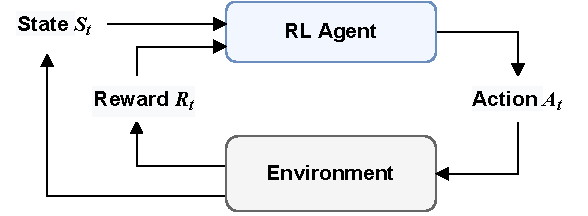
\includegraphics[width=0.5\textwidth]{RL-loop.pdf}
	\caption{Reinforcement Learning}
	\label{fig:RL-loop}
\end{figure}

Introduced in 1992, the REINFORCE algorithm \citep{REINFORCE-williams1992} is considered as a basic reinforcement learning algorithm. It is a policy-based, on-policy algorithm, capable of handling both discrete and continuous observation and action domains. In practice the REINFORCE algorithm is considered as a ``weak'' algorithm and superseded by several algorithms developed since. Most notably the Q-Learning and its deep-neural network version, the DQN \citep{DQN-mnih2013}, followed by Actor-Critic \citep{A2C-mnih2016} and one of the most robust modern-day algorithms, the PPO \citep{PPO-schulman2017}.

While most studies on RL algorithms are evaluated on Open AI Gym environments, our experiments cover the predictive maintenance problem using a custom built environment. Also, our study focuses on the earliest RL algorithm, the REINFORCE. This is often neglected by studies, as it is considered an early and weak algorithm. In the industry the milling tool is replaced after a set threshold. We use this ``deterministic preventive maintenance'' policy as the baseline for comparing the RL algorithm policy. 

Our systematic evaluation, based on levels of environment difficulty, different bench-mark datasets and varying noise levels allow a broader, more robust, comparison of the algorithms. Finally, we conduct statistical tests to ensure a robust statistical-evidence based conclusion. Based on experiments we show that REINFORCE works surprisingly well on tool-replacement precision and F-beta (0.5), over all the variants. The recall and F1-score are better or at-par with the advanced algorithms.\\

The main \textbf{contributions} of this research are:
\begin{enumerate}
	\item Contributes to the broader goal of AutoML for PdM using RL
	\item Research targeted toward the industrial practitioner not accustomed to complex hyper-parameter tuning of RL algorithms
	\item Design and implement an RL environment for predictive maintenance of a milling machine.
	\item Rigorous evaluation of four standard RL algorithms.
	\item Use of simple performance evaluation statistical measures and plots that industrial practitioners are normally used to.
\end{enumerate} 

The rest of the paper is structured as follows: In the next section we survey some related work and provide the necessary technical background describing the algorithms studied in this research. Section \ref{sec:Method} discusses implementation details of the REINFORCE algorithm and the predictive maintenance environment followed by the methodology adopted for training, testing and evaluation. Section \ref{sec:Results} presents the results of the experiments, that are discussed in Section \ref{sec:Discussion}. Finally, we summarize and draw conclusions in Section \ref{sec:Conclusion}.

\section{Related work and background}\label{sec:SLR}
\subsection{Literature Review}
Automated machine learning (AutoML) for predictive maintenance has been studied by only few researchers. All the 9 articles found use supervised machine learning. \cite{AutoML-Larocque} use signal processing to standardize data followed by AutoML to select top performing models. \cite{AutoML-Hadi} use AutoML to accurately identify various types of faults in ball bearings, while \cite{AutoML-Maurer} has studied use of AutoML on log-data generated by production lines for performing preventive maintenance. We did not find any work that applied AutoML for RL algorithms in the PdM context. 

Significant work has been conducted in the application of RL for predictive maintenance \citep{Panzer2021, Erhan2021, siraskar2023}, in general. However, we did not find\footnote{Search terms: \texttt{"reinforcement learning AND tool wear AND maintenance"}. As of: 10-Jul-2023.} any work done for predictive maintenance of \textit{milling machines} across three major journal index services\footnote{IEEE Xplore\texttrademark{}, Scopus\texttrademark{} and Web Of Science\texttrademark{}}. % $$$ Note: 1 article returned (\cite{dai2021reinforcement}) is NOT predictive maintenance - but clamping position optimization. 
While RL is not, traditional machine learning methods \textit{have} been applied; for example \cite{Qin2023} and \cite{Qiang2023} apply tool-wear law and physics based models before applying ML. \cite{Twardowski2023} and \cite{Denkena2023} use data gathered by sensors. While \cite{Twardowski2023} use two different classification trees, \cite{Denkena2023} use data recorded on other similar machines for building ML models. \cite{oshida2023development} proposes real-time tool wear detection using a stacked LSTM\footnote{long short-term memory networks} encoder-decoder model for anomaly detection as a mechanism to address predictive maintenance.  

Research work focusing of comparing experimental and empirical analysis of various RL algorithms, has been limited to using standard benchmark OpenAI Gym environments. \cite{sandeep2022experimental} documents experimental evaluation of four policy-gradient and actor-critic algorithms PPO, SAC, DDPG and A2C using OpenAI Gym environments such as the Pendulum, Mountain Car, Bipedal Walker, Lunar Landing and Atari 2600 game environments. \cite{Krishna2020} evaluate DQN, DoubleDQN, A2C, REINFORCE and PPO using Cartpole, Space Invaders and the Lunar Lander. \cite{dulac2021, dulac2020empirical} are significant contributions toward analyzing empirical studies directed toward \textit{real-world} challenges. They apply real-world design concepts on the Cartpole and other complex environments such as humanoid and walkers from the Real-World Reinforcement Learning (RWRL) Suite\footnote{Link to RWRL >>   \href{https://github.com/google-research/realworldrl_suite}{link}}. These environments are then evaluated for multiple RL algorithms such as, REINFORCE, Trust Region Policy Optimization (TRPO) and Deep Deterministic Policy Gradient (DDPG). 

\cite{dulac2021, henderson2018deep} tackle RL for continuous control. \cite{henderson2018deep} evaluate DDPG, ACKTR, TRPO and PPO on complex MuJoCo\footnote{\href{https://mujoco.org/}{MuJoCo} provids environments for studying Multi-Joint dynamics with Contact} environments such as the HalfCheetah, Hopper, Walker and Swimmer. Similar to our research, they used the OpenAI baseline implementations of RL algorithms for the experiments and evaluation. \cite{ford2022cognitive} is experimental evaluation we found that was based on real-world application. They compare DQN, A2C and PPO for choosing the operational radio frequency (RF) mode for a multi-function RF system and go on to suggest that PPO is the best.

The survey shows that most existing work use standard OpenAI Gym environments, which although necessary for bench marking performance, do not provide coverage of industrial predictive maintenance. In Section \ref{sec:Implementation} we attempt to bridge this gap by implementing a custom built environment.

\subsection{Technical Background}

\subsubsection*{Key concepts of RL}
A task is a goal we set for our agent to learn. In our case the agent must learn to optimally predict the replacement of the tool. Frequent tool replacement increases down-time while delaying it results in inferior work piece quality. In Fig. \ref{fig:RL-loop} the agent interacts with the environment by performing an action ($a \in \mathcal{A}$), which then alters the state of the environment to one of many states ($s \in \mathcal{S}$). The resulting state is determined by a state-transition probabilities ($\mathcal{P}$) since RL is founded on Markov Decision Process (MDP) theory. The new state provides a feedback via a reward ($r \in \mathcal{R}$). Higher positive rewards ``reinforce'' good behavior. Performing this over thousands of episodes with the objective of maximizing the total rewards $R$, enables the agent to develop a policy $\pi$ which is essentially a mapping of the optimal action to perform, given a certain state.

A \textbf{value function} computes how good a state or an action is by predicting future rewards, also known as a ``return'' $G_t = R_{t+1} + \gamma R_{t+2} + \dots = \sum_{k=0}^{\infty} \gamma^k R_{t+k+1}$. $\gamma \in [0, 1]$ facilitates discounting i.e. applying less weight to future rewards. 

Value functions can be represented by \textbf{state-value} $V_{\pi}(s)$ of a state $s$ as the expected return: $V_{\pi}(s) = \mathbb{E}_{\pi}[G_t \vert S_t = s]$; or an \textbf{action-value} function of a state-action pair as $Q_{\pi}(s, a) = \mathbb{E}_{\pi}[G_t \vert S_t = s, A_t = a]$.


%\textbf{Algorithm timelines}
%\begin{itemize}
%	\item 1947: Monte Carlo Sampling
%	\item 1959: Temporal Difference Learning
%	\item 1989: Q-Learning
%	\item 1992: REINFORCE
%	\item 2013: DQN
%	\item 2016: A3C
%	\item 2017: PPO 
%\end{itemize}

With a brief overview of RL, we now briefly touch upon the core ideas of the four algorithms we experimented with.

\subsubsection*{Deep Q-Network (DQN)}
Deep Q-Network \citep{DQN-mnih2013} significantly improved the earliest RL algorithm, Q-learning, by introducing neural networks to learn policies for high-dimension environments with two novel strategies to significantly stabilize learning -- an ``experience replay buffer'' and a target network that was frozen and only periodically updated. Equation (\ref{eq:DQN}) shows the DQN loss function where $D$ is the replay memory and is sampled using a uniform distribution $U(D)$, $Q(s, a; \theta)$ is the function parameterized with $\theta$, that helps compute the Q values and $\theta^{-}$ represents parameters of the frozen target Q-network.

\begin{equation}
	\mathcal{L}(\theta) = \mathbb{E}_{(s, a, r, s') \sim U(D)} \Big[ \big( r + \gamma \max_{a'} Q(s', a'; \theta^{-}) - Q(s, a; \theta) \big)^2 \Big]
	\label{eq:DQN}
\end{equation}

\subsubsection*{Advantage Actor Critic (A2C)}

A2C is a variant of Asynchronous Advantage Actor Critic (A3C) \citep{A2C-mnih2016}, and uses multiple computation workers to avoid the use of a replay buffer. A2C is a policy-gradient actor-critic algorithm. The policy-gradient family of algorithms strive to model and optimize the policy directly. Actor-critic structures consist of two networks -- a critic that updates function parameters $w$ of the value function (i.e either $Q_w(a \vert s)$ or $V_w(s)$); and an actor that updates the policy parameters $\theta$ for $\pi_\theta(a \vert s)$, following the direction computed by critic. Actors therefore learn the parameterized policy $\pi_{\theta}$ using the policy-gradient as shown in (\ref{eq:A2C}). 
\begin{equation}
	\nabla_ \theta J(\pi_\theta) = \mathbb{E}_t \; [ \; A^\pi_t \; \nabla_\theta \ln \pi_\theta(a_t \vert s_t) \;]
	\label{eq:A2C}
\end{equation}
Where the advantage function $A^\pi_t (s_t, a_t)$ measures how good or bad the action is w.r.t. policy's average, for a particular state, using (\ref{eq:A2CAF}).
\begin{equation}
	A^\pi_t (s_t, a_t) = Q^\pi (s_t, a_t) - V^\pi (s_t)
	\label{eq:A2CAF}
\end{equation}

\subsubsection*{Proximal Policy Optimization (PPO)} 
\cite{PPO-schulman2017} formulated PPO which is often considered as the most robust of the RL algorithms. PPO is policy-gradient method based on TRPO (Trust region policy optimization) by \cite{TRPO-schulman2015}, where the main idea is the use of a trust region to improve training stability by avoiding updates to parameters that vastly change the policy at a particular time step. TRPO ensures this by using a divergence constraint on the magnitude of policy update. If $r(\theta)$ (\ref{eq:rPPO}) represents the ratio of probabilities between policies of previous and current iteration, then the objective function of TRPO is given by (\ref{eq:TRPO}), where $\hat{A}$ represents the estimated advantage function.
\begin{equation}\label{eq:rPPO}
	r(\theta) = \frac{\pi_\theta(a \vert s)}{\pi_{\theta_\text{old}}(a \vert s)}
\end{equation}
\begin{equation}\label{eq:TRPO}
	J^\text{TRPO} (\theta) = \mathbb{E} [ r(\theta) \hat{A}_{\theta_\text{old}}(s, a) ]
\end{equation}

PPO extends TRPO by additionally imposing a regional constraint. It prevents large updates by forcing the ratio $r(\theta)$ to stay within a small interval $[1-\epsilon, 1+\epsilon]$, around $1.0$, by use of a hyper-parameter $\epsilon$.
\begin{equation}
	J^{CLIP} (\theta) = \mathbb{E}_t \; [ \; min (r_t(\theta) A^{\pi_{\theta_{old}}}_t, clip(r_t(\theta), 1-\epsilon, 1+\epsilon) A^{\pi_{\theta_{old}}}_t)]
	\label{eq:PPO}
\end{equation}

\subsubsection*{REINFORCE} 
The REINFORCE algorithm, invented by \cite{REINFORCE-williams1992}, is an early algorithm that directly learns a policy $\pi_\theta$ to produce action probabilities from states. Actions that cause favorable states are positively reinforced thereby increasing their probability of occurrence. Conversely, those resulting in unfavorable states are penalized.

The objective function (\ref{eq:REINFORCE-obj}) that the agent attempts to maximize is defined as the expected return over many trajectories sampled from the policy.
\begin{equation}\label{eq:REINFORCE-obj}
	\max_{\theta} J(\pi_{\theta}) = \mathop{\mathbb{E}}_{\tau \sim \pi_\theta} [R(\tau)]
\end{equation}

REINFORCE uses policy gradient to update the action probabilities.
\begin{equation}
	\nabla_ \theta J(\pi_\theta) = \mathbb{E}_t \; [ \; R_t(\tau) \; \nabla_\theta \ln \pi_\theta(a_t \vert s_t) \;]
	\label{eq:REINFORCE}
\end{equation}

\subsubsection*{Stable-Baselines3}
Stable-Baselines3 (SB3) \cite{SB3-paper} provides robust open source implementations of many reinforcement learning algorithms. The core algorithms of Stable-Baselines3 are completely refactored PyTorch implementations of Open AI baselines \citep{OpenAI-baselines}. \cite{SB3-PPO-implementation} describes the 37 PPO implementation details that SB3 carried out and demonstrates the complexity depth of their implementations.

As of 10-Jul-2023, 13 algorithms have been implemented \citep{SB3-algorithms}. REINFORCE has \textit{not} been implemented. For this research we use the \textit{default} SB3 implementations of DQN, A2C and PPO and compare its performance to a na\"ive custom implementation of the REINFORCE algorithm. %SB3 is popular among the RL community\footnote{As of 27-Jun-2023, it had 6k+ stars and 424 closed pull requests}.

\section{Methodology}\label{sec:Method}
\subsection{Implementation details}\label{sec:Implementation}
Reinforcement learning requires an environment to function. In this section we describe the custom milling environment we built, which allows our agent to learn a policy for tool replacement. Figure \ref{fig:environments} shows the stepped approach used to generate the \textit{fifteen} environments, of varying complexity, to evaluate the agents. In this section we describe the approach used to model and simulate tool-wear and hence generate wear data followed by actual tool wear data. We then describe the elements of environment design i.e. state, reward functions. The Python code used for this research is uploaded to GitHub at \href{https://github.com/Rajesh-Siraskar/Empirical_Study_REINFORCE}{URL}.  % $$$ we follow the procedure in \cite{graesser2019} pg 289 Part iv, ch14-15.
\begin{figure}[ht]
	\centering
	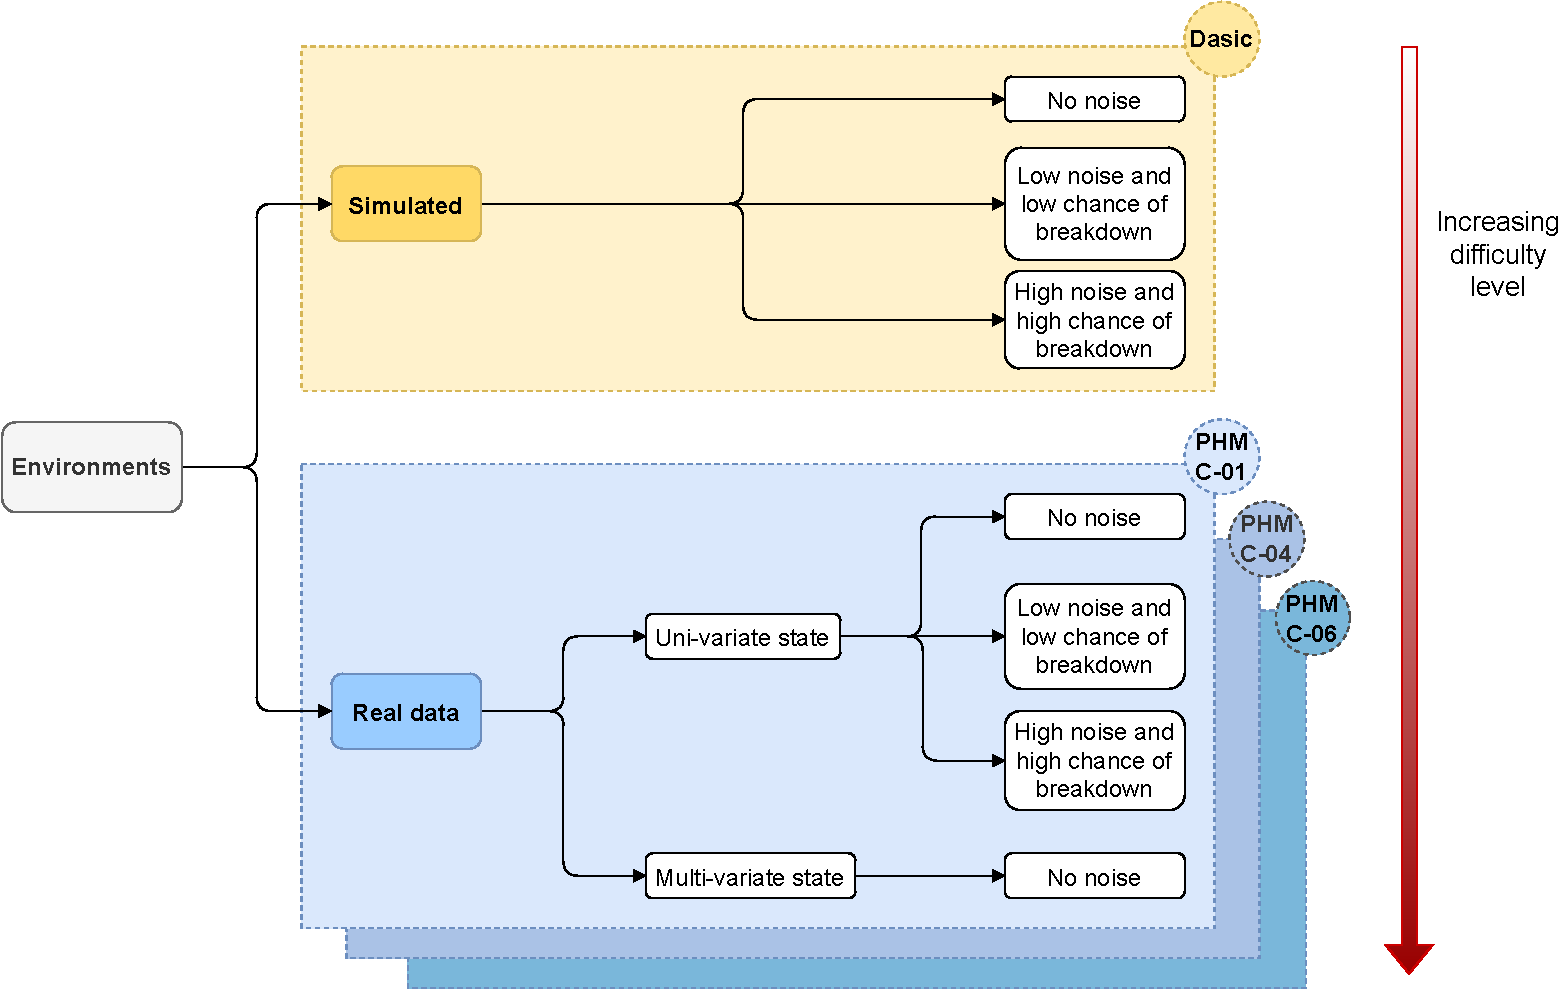
\includegraphics[width=\textwidth]{Environments.pdf}  
	\caption{The fifteen different environments used for evaluation}
	\label{fig:environments}
\end{figure} 

\begin{figure}[ht]
	\begin{subfigure}[b]{0.5\textwidth}
		\centering
		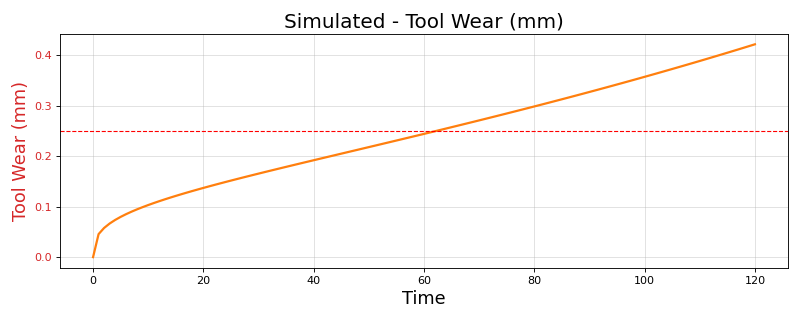
\includegraphics[width=\textwidth]{Simulated_wear_plot.png}  
		\caption{Simulated wear data}
		\label{fig:simulated}
	\end{subfigure}
	\hfill
	\begin{subfigure}[b]{0.5\textwidth}
		\centering
		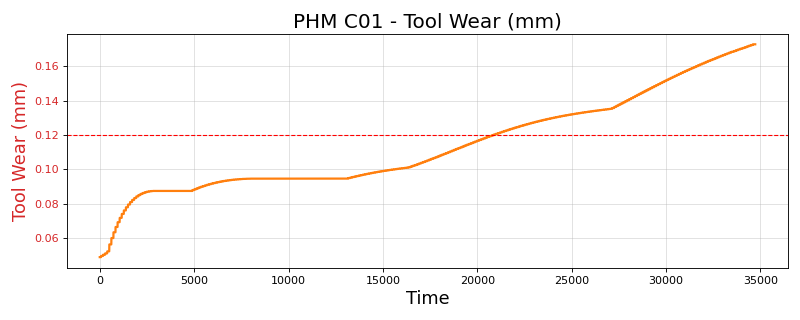
\includegraphics[width=\textwidth]{PHM_C01_wear_plot.png}  
		\caption{PHM C01 wear data}
		\label{fig:C01}
	\end{subfigure} \par\bigskip
	
	\begin{subfigure}[b]{0.5\textwidth}
		\centering
		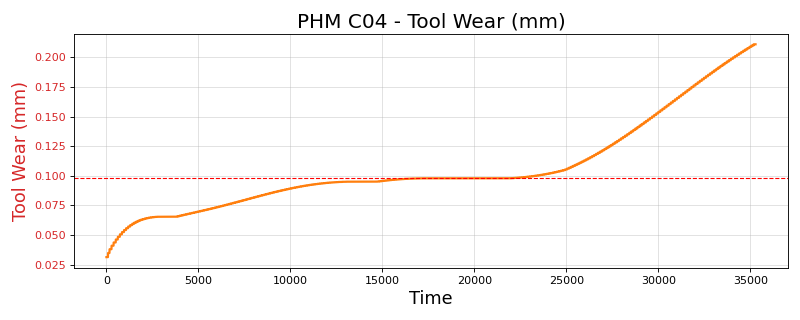
\includegraphics[width=\textwidth]{PHM_C04_wear_plot.png}  
		\caption{PHM C04 wear data}
		\label{fig:C04}
	\end{subfigure}
	\hfill
	\begin{subfigure}[b]{0.5\textwidth}
		\centering
		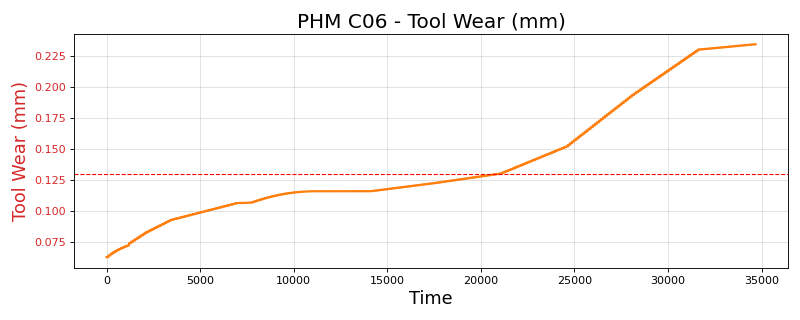
\includegraphics[width=\textwidth]{PHM_C06_wear_plot.png}  
		\caption{PHM C06 wear data}
		\label{fig:C06}
	\end{subfigure} 
	\label{fig:tool-wear-plots}
	\caption{Tool wear data. Red dotted line indicates the wear threshold beyond which tool is replaced.}
\end{figure}

\subsubsection*{Simulating tool-wear}
\cite{dasic2006} provide a parameterized power-exponential function for modeling tool wear (\ref{eq:Dasic}), where $VB$ represents the flank wear in mm.
\begin{equation}
	VB = a \cdot t^{b_1} \cdot e^{b_2 \cdot t} \Big|_{t=t_0}^{t=t_1}
	\label{eq:Dasic}
\end{equation}

We used the parameter values provided in the paper $a=0.08257, b1=0.3342, b2=0.03147$; and simulated 121 data points. Fig. \ref{fig:simulated} shows the tool wear simulated using (\ref{eq:Dasic}) with the red dotted line indicating the wear threshold beyond which tool is replaced. This provided the mechanism to simulate the tool wear based \textbf{univariate state}. We then add two further levels of increased complexity using noise and a chance of breakdown. This gives us three distinct environments. 

\subsubsection*{Actual tool wear data}
The IEEE DataPort hosts the tool wear data obtained from a high-speed CNC milling machine, \citep{NUAA-dataset}. C01, C04 and C06 datasets are suggested as benchmark for machine learning training and were the ones we used. The data consists of seven columns corresponding to dynamometer measuring force (N) in X, Y and Z dimensions; accelerometer measuring vibration (g) in X, Y and Z dimensions and finally acoustic emission data as AE-RMS (V). A separate file contains tool wear data in mm. Figures \ref{fig:C01}, \ref{fig:C04} and \ref{fig:C06} show the tool wear for the three datasets. We use the real data to create two state designs, an univariate state consisting of only the tool wear and a \textbf{multivariate} state designed using all the additional seven sensor values. As for the simulated case, the complexity of the \textit{univariate} state is increased using two levels of noise and break-down parameters. The multivariate state is complex in itself, Fig. \ref{fig:PHMMSdata}, and we use the natural (without noise) form.

\begin{figure}[ht]
	\centering
	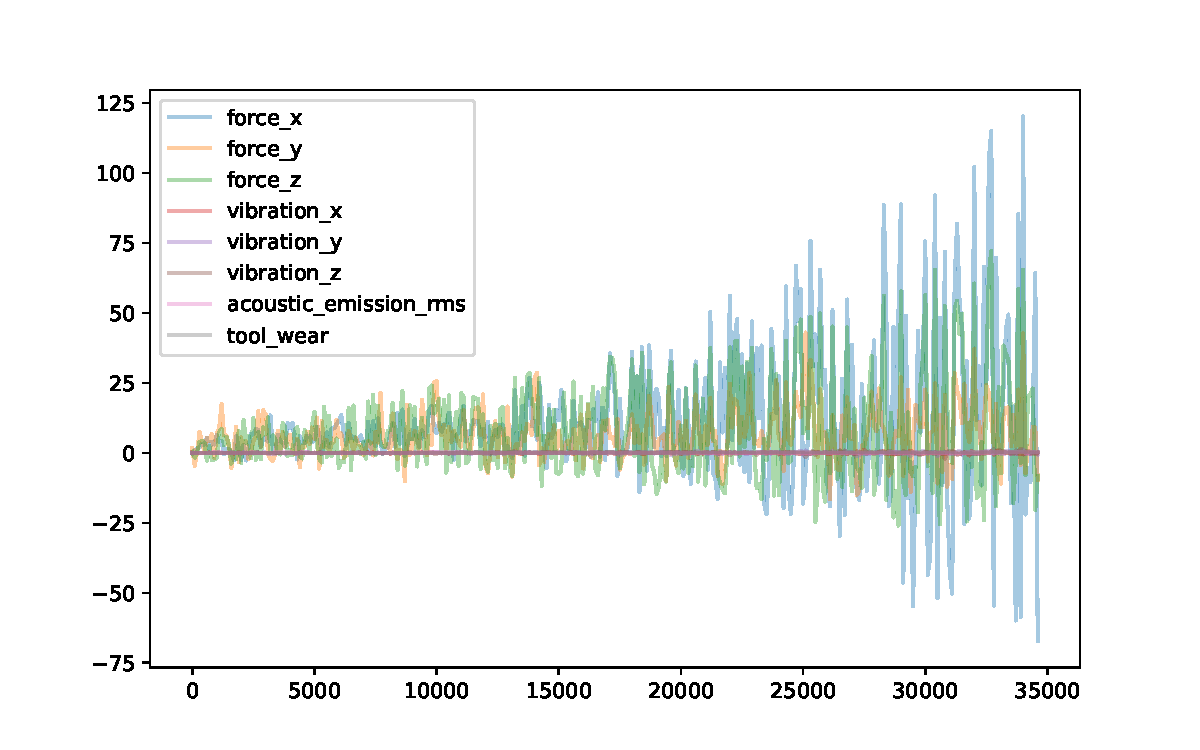
\includegraphics[width=0.8\textwidth]{PHMMSdata.pdf}  
	\caption{PHM C06: multivariate data}
	\label{fig:PHMMSdata}
\end{figure} 

In RL state variables are often normalized to improve stability and convergence. Both the simulated and real data was normalized using min-max scaling such that the tool wear and other state features, $x \in [0,\;1] \subset \mathbb{R} $. We will see next how this allows adding white noise of similar magnitudes across different PHM datasets.

\subsubsection*{Adding noise and chance of break-down}
Fig. (\ref{fig:noise}) shows the effect of adding two levels of noise. ``Low noise'' is obtained by adding Gaussian noise with an order of magnitude of $-3$ i.e. between $[0.0, 0.001]$ and ``high noise'' is of order $-2$ i.e. between $[0.0, 0.01]$. Since the tool wear data is normalized this adds significant perturbations as seen in Fig. (\ref{fig:LBD}) and (\ref{fig:HBD}). The noise affects the tool replacement decision (solid blue line) around the replacement threshold (dotted red line). The \textit{human} preventive maintenance policy replaces the tool if the wear exceeds the threshold and this decision boundary oscillates due to the noise. One can see that in the case of no noise (Fig. \ref{fig:NBD}), the decision boundary is clean.

\begin{figure}[htbp]
	\begin{subfigure}[b]{\textwidth}
		\centering
		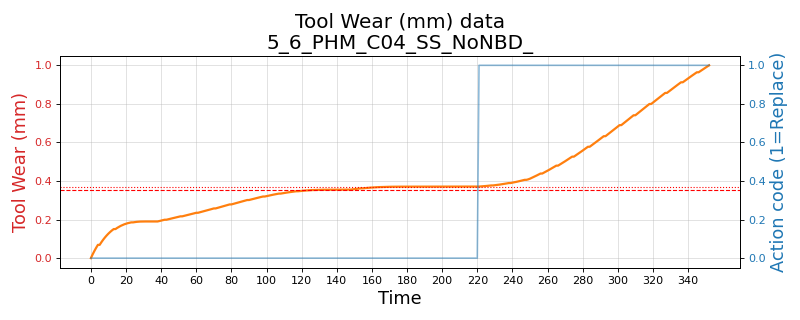
\includegraphics[width=0.65\textwidth]{PHM_C04_NoNBD_wear_plot.png}  
		\caption{No noise}
		\label{fig:NBD}
	\end{subfigure}
	\begin{subfigure}[b]{\textwidth}
		\centering
		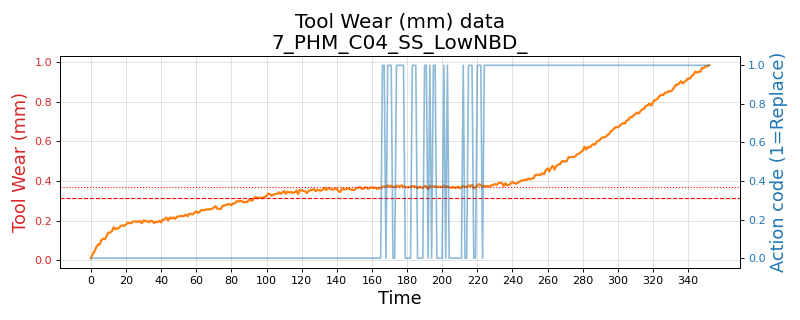
\includegraphics[width=0.65\textwidth]{PHM_C04_LowNBD_wear_plot.png}  
		\caption{Low noise}
		\label{fig:LBD}
	\end{subfigure}
	\begin{subfigure}[b]{\textwidth}
		\centering
		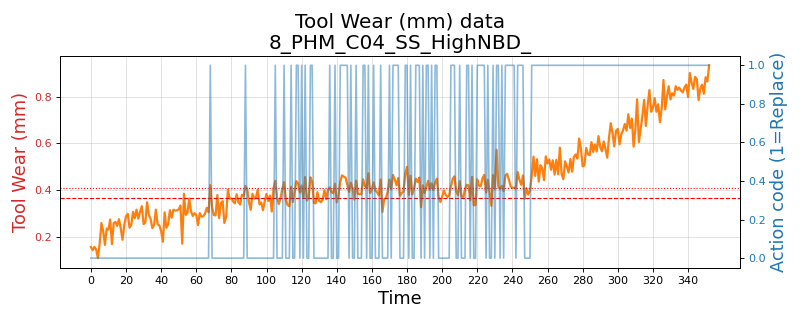
\includegraphics[width=0.65\textwidth]{PHM_C04_HighNBD_wear_plot.png}  
		\caption{High noise}
		\label{fig:HBD}
	\end{subfigure}
	\caption{PHM C04 tool wear data and the effect of noise.}
	\label{fig:noise}
\end{figure}

Break down occurs due to excessive tool use and can often occur randomly. In conjunction with Guassian noise this complexity is added for the univariate state based environments. For the low-noise variant we add a ``low chance'', 5\%, of break down and for the high noise variant we add a higher chance of 10\%. Sampled from a uniform distribution, the probability of break down is checked against this ``chance'' threshold and the episode is terminated if less than. This is seen in line 9 of the code in Listing \ref{lst:SSStep}. 

Table \ref{tbl:ListEnvironments} summarizes the 15 environment variants and their three logical groups: (1) Simulated 1-3 (2) Real data -- simple univariate environment (4-12) and Real data -- simple multivariate (13-15).

\begin{table*}
	\sffamily
	\rowspace{1.3}
	\begin{tabular}{@{}r l rr@{}} \arrayrulecolor{black!40}\toprule 
		 & Environment variant & Noise factor & Breakdown chance \\ \midrule
		 & \multicolumn{3}{l}{\textbf{Simulated}}\\
		1 & Simulated - No noise  & None & None \\
		2 & Simulated - Low noise & 1e-3 & 0.05 \\
		3 & Simulated  - High noise & 1e-2 & 0.10 \\ \midrule
		\rule{0pt}{1.5\normalbaselineskip}
		 & \multicolumn{3}{l}{\textbf{Real data -- simple univariate}} \\
		4 & PHM C01 SS (simple, univariate) - No noise & None & None \\
		5 & PHM C01 SS (simple, univariate) - Low noise & 1e-3 & 0.05 \\
		6 & PHM C01 SS (simple, univariate) - High noise & 1e-2 & 0.10 \\ \hdashline
		
		7 & PHM C04 SS (simple, univariate) - No noise & None & None \\
		8 & PHM C04 SS (simple, univariate) - Low noise & 1e-3 & 0.05 \\
		9 & PHM C04 SS (simple, univariate) - High noise & 1e-2 & 0.10 \\ \hdashline
		
		10 & PHM C06 SS (simple, univariate) - No noise & None & None \\
		11 & PHM C06 SS (simple, univariate) - Low noise & 1e-3 & 0.05 \\
		12 & PHM C06 SS (simple, univariate - High noise & 1e-2 & 0.10 \\ \midrule
		
		\rule{0pt}{1.5\normalbaselineskip}
		& \multicolumn{3}{l}{\textbf{Real data -- complex multivariate}}\\
		13 & PHM C01 MS (complex, multivariate) - No noise & None & None \\
		14 & PHM C04 MS (complex, multivariate) - Low noise & 1e-3 & 0.05 \\
		15 & PHM C06 MS (complex, multivariate) - High noise & 1e-2 & 0.10 \\ \bottomrule
	\end{tabular}
	\caption{List of the fifteen environments and their categorization}
	\label{tbl:ListEnvironments}
\end{table*}

\subsubsection*{Actions}
The choice of action is binary and represented by $\text{ACTION} \in [0, 1]$, where $0$ represents continuation of milling operation ($\text{CONTINUE}$), while $1$ represents the action of replacing the tool ($\text{REPLACE\_TOOL}$).

\subsubsection*{Reward function}
The reward function (\ref{eq:RewardFunction}) drives the learning process. Code implementation is seen in Listing \ref{lst:SSStep}. There are three important phases where reward (or penalty) is provided as feedback. $R_1$, $R_2$ and $R_3$ are constants that determine the magnitude of reward. The first condition is when the current state of wear $w(s_t)$ is less than the threshold $W_T$, and a desirable condition, hence the reward is positive. The formulation allows higher reward to be collected the closer it is to threshold, but not allowing it to cross it. If it does, the agent is penalized (negative reward) by a magnitude of $R2$ and once again the farther away it is from the threshold i.e. a highly deteriorated tool the larger the penalty. To avoid this ``bad" state, the agent must learn to replace the tool; represented by the third condition. Tool replacement implies a direct cost (that of the tool) and a much higher and significant downtime ``cost''. To ensure the agent learns not to replace unnecessarily, we ``penalize'' it. It is important to note that the last condition in (\ref{eq:RewardFunction}) is an ``incremental addition", the first two conditions are mutually exclusive and evaluated first, followed by the last condition which is incrementally added on whatever reward is collected in the previous condition. The agent then tries to balance these three condition, such that it maximizes its total return, over time.
\begin{equation}
	R_t \;\;=\;\;
	\begin{cases}
		\;\;  +R_1 \times t, & \quad if \;\; w(s_t) < W_T\\
		\;\;  -R_2 \times t, & \quad if \;\; w(s_t) \ge W_T\\
		\;\; \mathrel{+}= -R_3, & \quad if \;\; \text{ACTION = REPLACE\_TOOL}\\
	\end{cases}
	\label{eq:RewardFunction}
\end{equation}

\subsubsection*{Environment feedback}
Figure \ref{fig:RL-loop} shows ``feedback'' that is important for the agent to learn from the action it takes. This is performed by the \texttt{step()} function in the environment code and the main parts are shown in Listing \ref{lst:SSStep}. At every time step an action is taken, the conditions (e.g. lines 2 and 8) of the resulting state evaluated for assigning a reward and then either proceeding or terminating the episode (e.g. lines 9 and 11).

\begin{lstlisting}[language=Python, label={lst:SSStep}, caption={Environment: Important implementation details of the 'step' function}]
# Termination condition
if self.ep_length >= self.max_operations:
	terminated = True
	self.reward = 0.0
	self.df_index = -1
	info = {'termination':'Max. milling operations crossed'}

elif (tool_wear > self.wear_threshold and 
	np.random.uniform() < self.breakdown_chance):
	terminated = True
	self.reward = 0.0
	self.df_index = -1
	info = {'termination':'Tool breakdown'}

else:
	terminated = False
	info = {'action':'Continue'}
	reward = 0.0
	
	if tool_wear < self.wear_threshold:
		reward += self.R1*self.df_index
	else:
		# Threshold breached. Farther away from threshold => more penalty
		reward += self.R2*self.df_index 
		
	# Based on the action = 1 replace the tool or if 0, continue with normal operation
	if action:
		reward += self.R3 
		self.df_index = -1 # Tool replaced - so roll back tool life
		self.ep_tool_replaced += 1 # Increment tool replaced count
		info = {'action':'Tool replaced'}
\end{lstlisting}

%\begin{lstlisting}[language=Python, label={lst:msstate}, caption={Multivariate state}]
%	def _get_observation(self, index):
%		next_state = np.array([
%		self.df['force_x'][index],
%		self.df['force_y'][index],
%		self.df['force_z'][index],
%		self.df['vibration_x'][index],
%		self.df['vibration_y'][index],
%		self.df['vibration_z'][index],
%		self.df['acoustic_emission_rms'][index],
%		self.df['tool_wear'][index]
%		], dtype=np.float32)
%	return next_state
%\end{lstlisting}
\subsubsection*{Network architecture and basic hyper-parameters}
For this research we implemented a na\"ive REINFORCE algorithm, with very simple network architectures. This was compared against \textit{default} implementations of the more advanced algorithms; DQN, A2C and PPO, from the Stable-Baselines3 library. Table \ref{tbl:network-architecture} shows a comparison of the network architecture and the basic common hyper-parameters.

\begin{small}
\begin{table*}\centering
	\sffamily
	\rowspace{1.5}
	\begin{tabular}[htbp]{L{2cm} R{2.5cm} R{2.5cm} R{2.5cm} R{3cm}}
		\arrayrulecolor{black!40}\toprule
		&\textbf{A2C}&\textbf{DQN}&\textbf{PPO}&\textbf{REINFORCE}\\ \midrule
		
		Network\par architecture&input dim x\par [64|Tanh x 64|Tanh]\par x output dim&input dim x\par [64|Tanh x 64|Tanh]\par x output dim&input dim x\par [64|Tanh x 64|Tanh]\par x output dim&input dim x\par [64|ReLU]\par x output dim\\
		Layers&2&2&2&1\\
		Units&64  x 64&64  x 64&64  x 64&64\\
		Activation&Tanh, Tanh&Tanh, Tanh&Tanh, Tanh&ReLU\\
		Optimizer&RMSprop&Adam&Adam&Adam\\ \midrule
		Learning rate&0.0007&0.0001&0.0003&0.01\\
		Gamma&0.99&0.99&0.99&0.99\\			
		\bottomrule
	\end{tabular}
	\caption{Comparing the network architecture and basic hyper-parameters across algorithms}
	\label{tbl:network-architecture}
\end{table*}
\end{small}
The REINFORCE uses a \textit{single} internal layer of 64 units. The default network architecture for all three SB3 algorithms (A2C/DQN/PPO) consists of \textit{two} fully connected layers with 64 units per layer \citep{SB3-DefaultNetwork}. While we used ReLU (rectified linear unit) as the activation function, the other three algorithms used hyperbolic tangent (Tanh).

\subsection{Training}
The training strategy must ensure a uniform comparison of the algorithms. We maintained the exact \textit{same} environment variant, wear dataset, noise parameter, probability of breakdown parameter, and the reward function parameters $R_1$, $R_2$ and $R_3$; across all four algorithms during a single training round. Our code is fairly automated and we used a configuration file to configure the training experiments and record the results. Fig. \ref{fig:exptconfig} shows the main columns of the configuration file we used.

As the wear data is time-series data, the training and test sets are created by systematic sampling. Simulated data and real tool-wear data (PHM) was randomly sampled at a certain frequency and down sampled into training and test sets.

\begin{figure}[ht]
	\centering	
	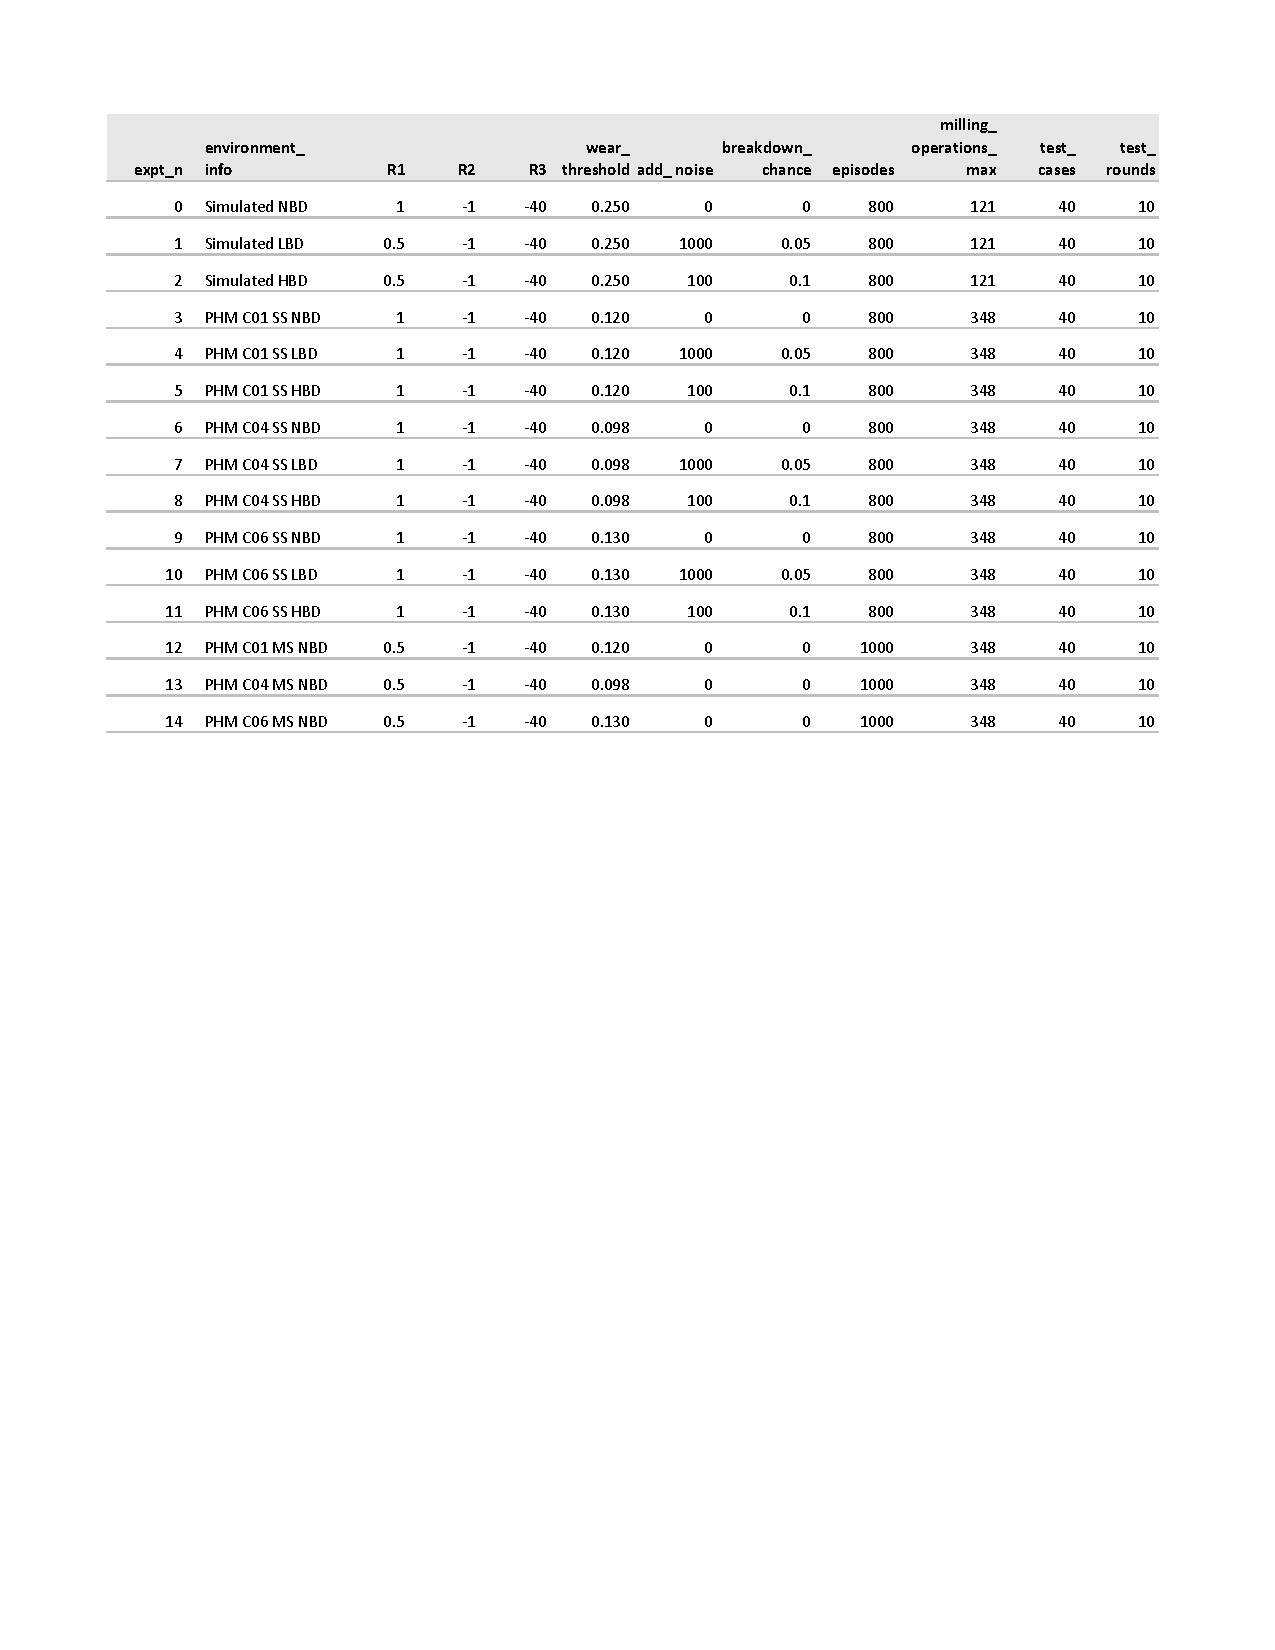
\includegraphics[width=\textwidth, trim={1.5cm 15cm 1cm 2cm}, clip]{images/TrainingPlots/Experiments_Sheet_select.pdf}  
	\caption{Configuring the experiments}
	\label{fig:exptconfig}
\end{figure}

The REINFORCE was trained for 800 episodes for the simulated and PHM univariate variants, for all three noise and breakdown levels (none, low and high) -- Table \ref{tbl:ListEnvironments} items 1-12. For the PHM multivariate variant Table \ref{tbl:ListEnvironments} items 13-15, REINFORCE was trained for 1000 episodes. SB3 algorithms were trained for 10,000 episodes for all variants. We ran ten rounds of training, tested each model generated and then averaged their results. Testing is explained in the next section while results are presented in Section \ref{sec:Results}.

\begin{figure}[ht]
	\begin{subfigure}[b]{0.5\textwidth}
		\centering
		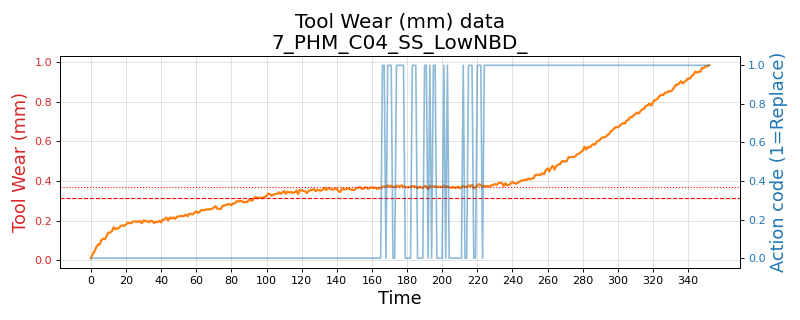
\includegraphics[width=\textwidth]{images/TrainingPlots/7_PHM_C04_SS_LowNBD__wear_plot.png}  
		\caption{PHM C04 wear data}
		\label{fig:C04wear}
	\end{subfigure}
	\hfill
	\begin{subfigure}[b]{0.5\textwidth}
		\centering
		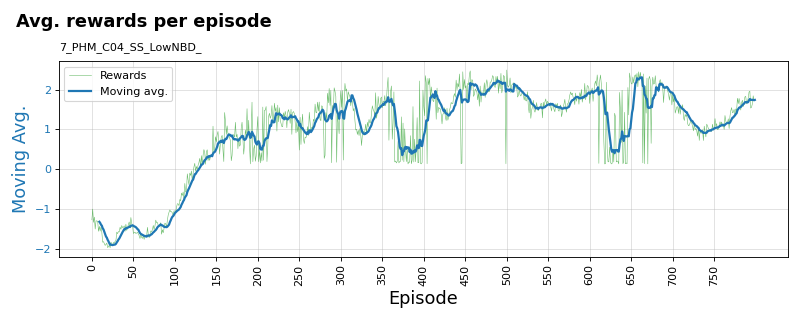
\includegraphics[width=\textwidth]{images/TrainingPlots/7_PHM_C04_SS_LowNBD__Avg_episode_rewards.png}  
		\caption{Average rewards per episode}
		\label{fig:C04rewards}
	\end{subfigure} \par\bigskip
	
	\begin{subfigure}[b]{0.5\textwidth}
		\centering
		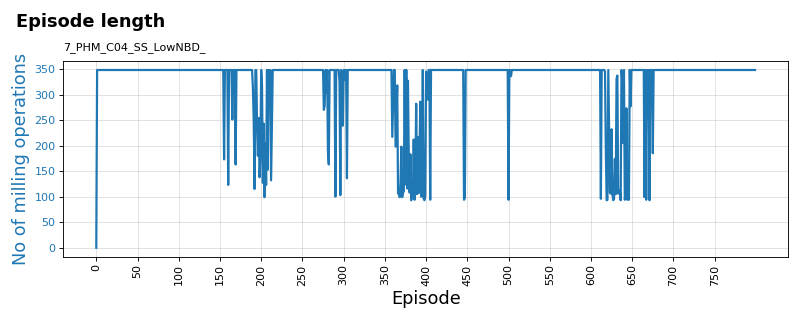
\includegraphics[width=\textwidth]{images/TrainingPlots/7_PHM_C04_SS_LowNBD__Episode_Length.png}  
		\caption{Episode length completed per episode}
		\label{fig:C04eplen}
	\end{subfigure}
	\hfill
	\begin{subfigure}[b]{0.5\textwidth}
		\centering
		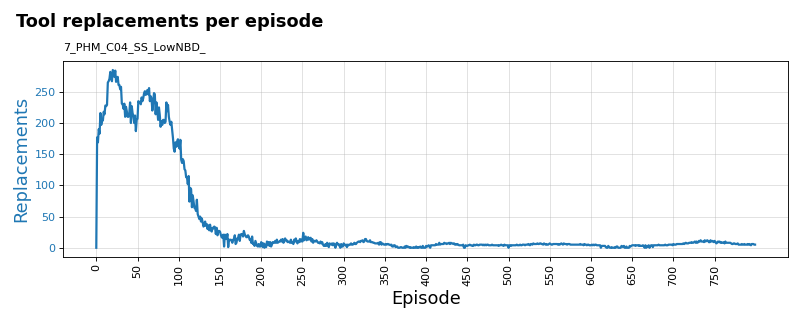
\includegraphics[width=\textwidth]{images/TrainingPlots/7_PHM_C04_SS_LowNBD__Tool_Replacements.png}  
		\caption{Tool replacements per episode}
		\label{fig:C04toolrep}
	\end{subfigure} 
	\caption{Training plots. Algorithm: REINFORCE. Dataset: PHM-C04. Variant: Univariate state, low-noise and low chance of breakdown.}
	\label{fig:C04trplots}
\end{figure}
Figure \ref{fig:C04trplots} shows the training plots for the algorithm of our interest -- REINFORCE. It displays how the wear plot looked for C04 with low noise and low chance of breakdown settings. The average rewards increase over the course of 800 episodes (Fig. \ref{fig:C04rewards}), the episode length demonstrates the complexity introduced by random breakdown (which abruptly terminates the episode). It is the tool replacement policy that is essentially of interest to the industrial practitioner, this decreases to optimal levels as the agent learns over time, as seen in Fig. \ref{fig:C04toolrep}. Similarly, Fig. \ref{fig:C06trplots} demonstrates the training for the PHM C06 dataset affected by high noise and higher breakdown probability. Finally, for the more complex multivariate state variant, the training plots are as seen in Fig. \ref{fig:C01trplots}; as we do not introduce noise or breakdown here, the episodes are always completed (Fig. \ref{fig:C01eplen}).

\begin{figure}[ht]
	\begin{subfigure}[b]{0.5\textwidth}
		\centering
		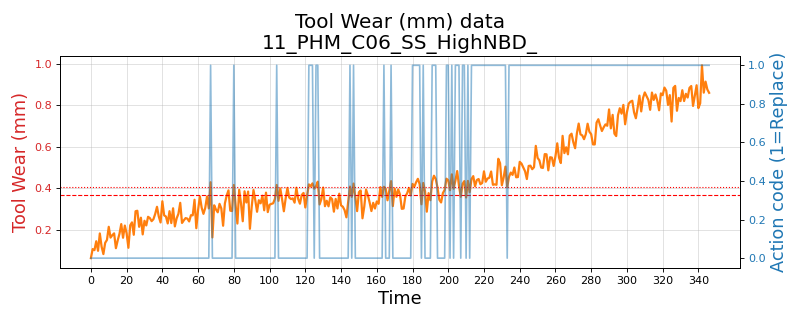
\includegraphics[width=\textwidth]{images/TrainingPlots/11_PHM_C06_SS_HighNBD__wear_plot.png}  
		\caption{PHM C06 wear data}
		\label{fig:C06wear}
	\end{subfigure}
	\hfill
	\begin{subfigure}[b]{0.5\textwidth}
		\centering
		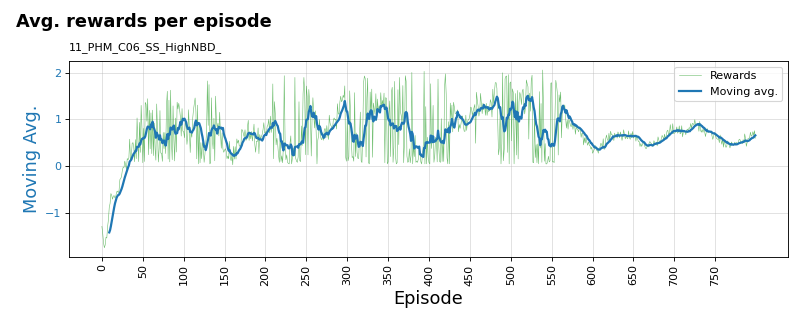
\includegraphics[width=\textwidth]{images/TrainingPlots/11_PHM_C06_SS_HighNBD__Avg_episode_rewards.png}  
		\caption{Average rewards per episode}
		\label{fig:C06rewards}
	\end{subfigure} \par\bigskip
	
	\begin{subfigure}[b]{0.5\textwidth}
		\centering
		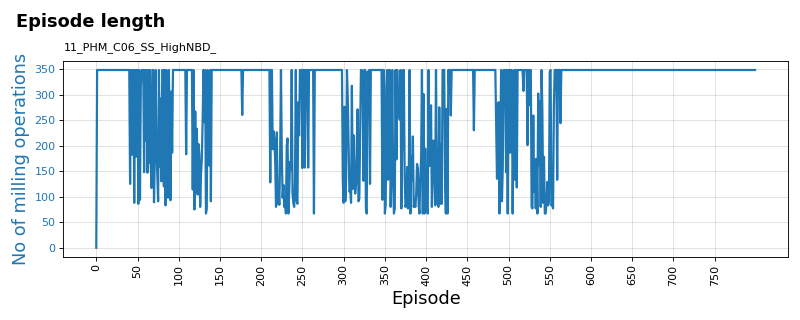
\includegraphics[width=\textwidth]{images/TrainingPlots/11_PHM_C06_SS_HighNBD__Episode_Length.png}  
		\caption{Episode length completed per episode}
		\label{fig:C06eplen}
	\end{subfigure}
	\hfill
	\begin{subfigure}[b]{0.5\textwidth}
		\centering
		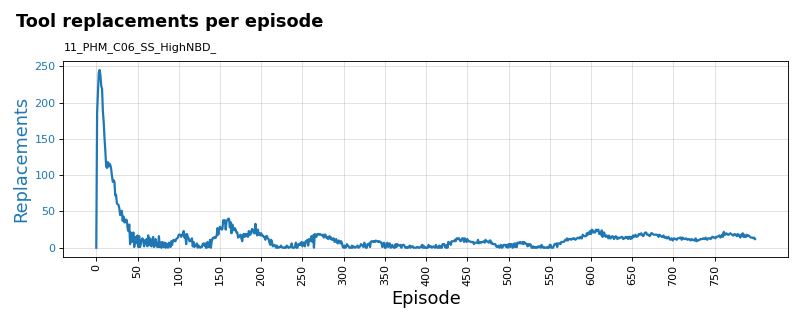
\includegraphics[width=\textwidth]{images/TrainingPlots/11_PHM_C06_SS_HighNBD__Tool_Replacements.png}  
		\caption{Tool replacements per episode}
		\label{fig:C06toolrep}
	\end{subfigure} 
	\caption{Training plots. Algorithm: REINFORCE. Dataset: PHM-C06. Variant: Univariate state, high-noise and high chance of breakdown.}
	\label{fig:C06trplots}
\end{figure}

\begin{figure}[ht]
	\begin{subfigure}[b]{0.5\textwidth}
		\centering
		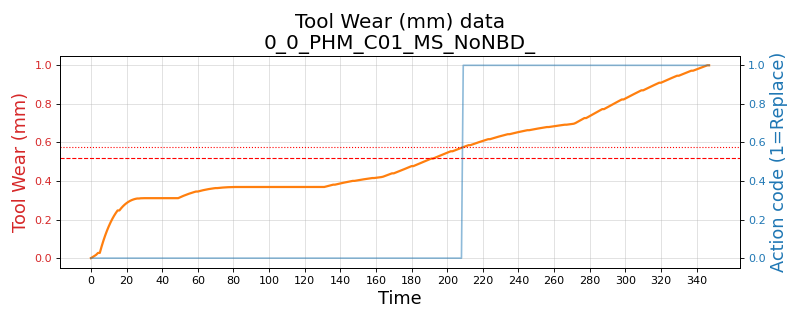
\includegraphics[width=\textwidth]{images/TrainingPlots/0_0_PHM_C01_MS_NoNBD__wear_plot.png}  
		\caption{PHM C01 wear data}
		\label{fig:C01wear}
	\end{subfigure}
	\hfill
	\begin{subfigure}[b]{0.5\textwidth}
		\centering
		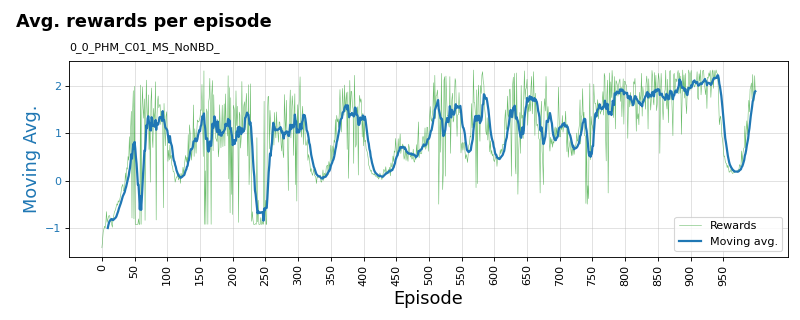
\includegraphics[width=\textwidth]{images/TrainingPlots/0_0_PHM_C01_MS_NoNBD__Avg_episode_rewards.png}  
		\caption{Average rewards per episode}
		\label{fig:C01rewards}
	\end{subfigure} \par\bigskip
	
	\begin{subfigure}[b]{0.5\textwidth}
		\centering
		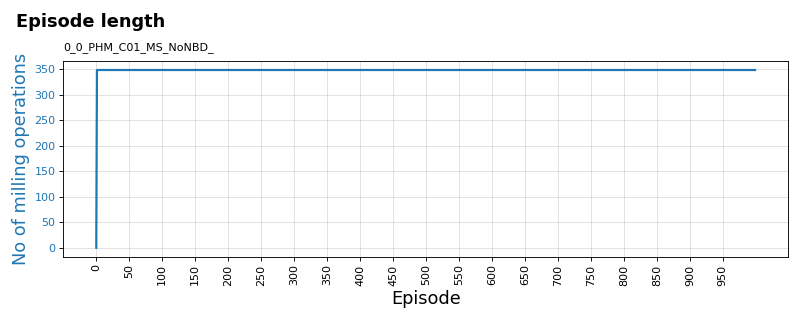
\includegraphics[width=\textwidth]{images/TrainingPlots/0_0_PHM_C01_MS_NoNBD__Episode_Length.png}  
		\caption{Episode length completed per episode}
		\label{fig:C01eplen}
	\end{subfigure}
	\hfill
	\begin{subfigure}[b]{0.5\textwidth}
		\centering
		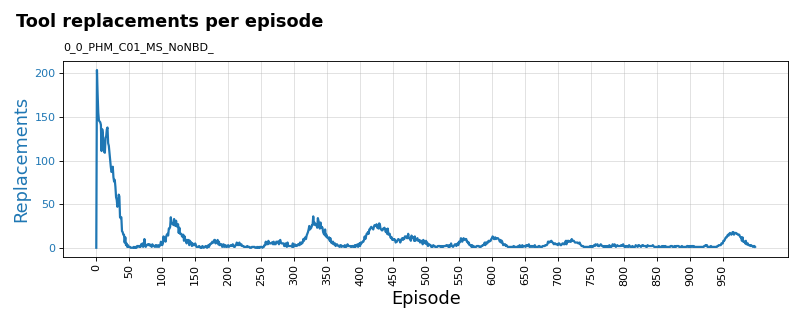
\includegraphics[width=\textwidth]{images/TrainingPlots/0_0_PHM_C01_MS_NoNBD__Tool_Replacements.png}  
		\caption{Tool replacements per episode}
		\label{fig:C01toolrep}
	\end{subfigure} 
	\caption{Training plots. Algorithm: REINFORCE. Dataset: PHM-C01. Variant: Multivariate state, No noise or breakdown.}
	\label{fig:C01trplots}
\end{figure}

\subsection{Testing and performance evaluation}
Testing was performed with data separate from the training data. 10 rounds of testing are performed, with a \textit{new} set of 40 test cases randomly sampled and frozen across all four algorithms. 

\subsubsection*{Evaluation metrics}
In our data, we indicate a tool replacement suggested by the human expert as 1, and a normal operation as 0. The human decision is based on ``preventive maintenance'' against a set threshold. In reality the threshold is based on several factors like materials of tool and work-piece, the duration of continuous operation, ambient conditions, ``cost'' of production downtime etc. Threshold could therefore vary significantly from one case to another.

We applied classification metrics to evaluate the RL agent decisions that suggest similar actions. These are simple to understand for the general industrial practitioners. 
\begin{figure}
	\begin{center}
		\sffamily
		\rowspace{1.6}
		\begin{tabular}{l|l|c|c|}
			\multicolumn{2}{c}{}&\multicolumn{2}{c}{\textbf{Human action}}\\
			\cline{3-4}
			\multicolumn{2}{c|}{}&Replace tool&Continue milling\\
			\cline{2-4}
			\multirow{2}{*}{\textbf{Agent action}}& Replace tool & $TP$ & $FP$\\
			\cline{2-4}
			& Continue milling& $FN$ & $TN$\\
			\cline{2-4}
		\end{tabular}
	\end{center}
	\caption{Confusion matrix }
	\label{fig:CM}	
\end{figure}
Classification metrics are based on the confusion matrix shown in Fig. \ref{fig:CM}. $TP$ represents true positive cases, where both the agent and human agree on replacing the tool. False positive $FP$ cases denote the agent falsely suggesting replacements. With false negative $FN$, the agent suggests to continue milling operation when a tool replacement would have helped. Precision (Pr), Recall (Rc) and F1-score metrics can then be computed as shown in (\ref{eq:metrics}).

\begin{equation}
	\text{Pr} = \frac{TP}{TP+FP}, \quad
	\text{Rc} = \frac{TP}{TP+FN}, \quad
	\text{F1-score} = 2 \times \frac{Pr \times Rc)}{(Pr + Rc)}
	\label{eq:metrics}
\end{equation}

\textbf{Tool replacement precision}: Timely replacements, $TP$, ensures work piece quality. While we desire high $TP$s, we do want to simultaneously drive down \textit{unnecessary} replacements and reduce costly production downtime, we therefore want lower $FP$s. The precision metric is therefore an ideal metric. 

While we prefer a high precision, we do want a reasonably high recall i.e. do not want to miss replacement opportunities (low $FN$s). The F1-score (\textit{true} harmonic mean of precision and recall) gives us a \textit{balanced} measure. Equation (\ref{eq:Fbeta}) provides a \textit{weighted} mechanism to provide a higher F-score for higher precision, by setting $\beta < 1.0$. For our evaluation we set $\beta$ to $0.5$.

\begin{equation}
	F_{\beta} = (1+\beta^2) \cdot \frac{Pr \times Rc)}{(\beta^2 \cdot Pr + Rc)}
	\label{eq:Fbeta}
\end{equation}

%\begin{verbatim}
%	env = MillingTool_SS_NT(df_train, WEAR_THRESHOLD_NORMALIZED, MILLING_OPERATIONS_MAX, ADD_NOISE, BREAKDOWN_CHANCE, R1, R2, R3)
%	
%	env_test = MillingTool_SS_NT(df_test, WEAR_THRESHOLD_ORG_NORMALIZED, MILLING_OPERATIONS_MAX, ADD_NOISE, BREAKDOWN_CHANCE, R1, R2, R3)
%\end{verbatim}

\section{Results}\label{sec:Results}
In the previous section we discussed the training and testing methods, as well as the evaluation metrics. Our automated code reads settings shown in Fig. \ref{fig:exptconfig} and creates 10 models. Each model is tested 10 times, with a fresh set of 40 randomly sampled points. The results are presented in this section.

We first present averaged metrics and averaged standard deviation of \textit{all} 15 variants in Table \ref{tbl:DetailedMetrics}, followed by category wise summary of results:
\begin{enumerate}
	\item Overall performance: Averaged over all 15 environments -- Table \ref{tbl:ListEnvironments}, items 1 to 15.
	\item Simulated environment: Averaged over 3 noise setting variants -- Table \ref{tbl:ListEnvironments}, items 1 to 3.
	\item Real data - simple univariate state: Averaged over 9 variants i.e. 3 PHM datasets (C01, C04 and C06) with 3 noise settings -- Table \ref{tbl:ListEnvironments}, items 4 to 12. 
	\item Real data - complex multivariate state: Averaged over 3 variants of PHM datasets (C01, C04 and C06) -- Table \ref{tbl:ListEnvironments}, items 13 to 15. 
\end{enumerate}
\newgeometry{margin=1cm} % Change margins for landscape table
\begin{landscape}\centering
	\begin{table*}
		\sffamily
		\rowspace{1.3}
		\begin{tabular}{@{}l rrrr c rrrr c rrrr c rrrr@{}} \arrayrulecolor{black!40}\toprule
			& \multicolumn{4}{c}{\textbf{REINFORCE}} & & \multicolumn{4}{c}{A2C} &
			& \multicolumn{4}{c}{DQN} & & \multicolumn{4}{c}{PPO} \\
			\cmidrule{2-5} \cmidrule{7-10} \cmidrule{12-15} \cmidrule{17-20}
			Environment &Prec. &Recall &F1 &F$_\beta$0.5 & &Prec. &Recall &F1 &F$_\beta$0.5 & &Prec. &Recall &F1 &F$_\beta$0.5 & &Prec. &Recall &F1 &F$_\beta$0.5\\ \midrule
			Simulated  - No noise &0.842 &0.878 &0.838 & 0.834 & & 0.424 &0.451 &0.423 &0.421 & &0.426 &0.674 &0.471 &0.410 & &0.504 &0.200 &0.271&0.360\\
			Simulated  - Low noise &0.777 &0.929 &0.834 & 0.796 & & 0.465 &0.423 &0.409 &0.427 & &0.421 &0.338 &0.270 &0.283 & &0.482 &0.236 &0.296&0.369\\
			Simulated  - High noise &0.798 &0.940 &0.851 & 0.816 & & 0.358 &0.281 &0.256 &0.272 & &0.447 &0.519 &0.380 &0.360 & &0.514 &0.207 &0.286&0.382\\ \midrule
			
			PHM C01 SS - No noise &0.478 &0.363 &0.400 & 0.439 & & 0.501 &0.500 &0.493 &0.496 & &0.472 &0.807 &0.568 &0.490 & &0.440 &0.417 &0.387&0.395\\
			PHM C01 SS - Low noise &0.507 &0.311 &0.332 & 0.383 & & 0.503 &0.598 &0.535 &0.513 & &0.393 &0.502 &0.351 &0.317 & &0.522 &0.338 &0.388&0.448\\
			PHM C01 SS - High noise &0.693 &0.562 &0.579 & 0.623 & & 0.266 &0.282 &0.267 &0.262 & &0.458 &0.525 &0.400 &0.384 & &0.456 &0.369 &0.372&0.400\\ \hdashline
			
			PHM C04 SS - No noise &0.751 &0.878 &0.784 & 0.757 & & 0.487 &0.442 &0.449 &0.463 & &0.439 &0.684 &0.472 &0.411 & &0.500 &0.510 &0.469&0.473\\
			PHM C04 SS - Low noise &0.662 &0.756 &0.672 & 0.657 & & 0.409 &0.455 &0.428 &0.416 & &0.411 &0.500 &0.370 &0.341 & &0.488 &0.280 &0.324&0.386\\
			PHM C04 SS - High noise &0.611 &0.713 &0.620 & 0.598 & & 0.518 &0.607 &0.552 &0.530 & &0.358 &0.451 &0.325 &0.294 & &0.428 &0.262 &0.286&0.333\\ \hdashline
			
			PHM C06 SS - No noise &0.830 &0.726 &0.754 & 0.792 & & 0.517 &0.509 &0.507 &0.511 & &0.360 &0.309 &0.256 &0.258 & &0.409 &0.248 &0.275&0.321\\
			PHM C06 SS - Low noise &0.205 &0.279 &0.228 & 0.212 & & 0.510 &0.577 &0.530 &0.516 & &0.434 &0.266 &0.266 &0.296 & &0.417 &0.181 &0.232&0.294\\
			PHM C06 SS - High noise &0.709 &0.843 &0.759 & 0.726 & & 0.316 &0.324 &0.311 &0.308 & &0.449 &0.518 &0.400 &0.375 & &0.388 &0.222 &0.265&0.317\\ \midrule
			
			PHM C01 MS - No noise &0.835 &0.652 &0.656 & 0.716 & & 0.461 &0.444 &0.397 &0.404 & &0.384 &0.558 &0.393 &0.348 & &0.513 &0.383 &0.416&0.460\\
			PHM C04 MS - No noise &0.739 &0.255 &0.359 & 0.494 & & 0.498 &0.589 &0.490 &0.470 & &0.323 &0.209 &0.160 &0.168 & &0.499 &0.393 &0.421&0.457\\
			PHM C06 MS - No noise &0.864 &0.356 &0.469 & 0.616 & & 0.501 &0.713 &0.578 &0.527 & &0.489 &0.705 &0.529 &0.479 & &0.523 &0.488 &0.485&0.498\\
			
			\bottomrule
		\end{tabular}
		\caption{Model performance comparison all variants of the environments, over 10 rounds of training.}
		\label{tbl:DetailedMetrics}
	\end{table*}
\end{landscape}
\restoregeometry % Restore margins after landscape table

\subsection{Overall summary performance}
\begin{table*}[!htb]\centering
	\sffamily
	\rowspace{1.3}
	\begin{tabular}{@{}l rr c rr c rr c rr@{}}
		\arrayrulecolor{black!40}\toprule
		& \multicolumn{2}{c}{Precision} & \phantom{i} & \multicolumn{2}{c}{Recall} & \phantom{i} & \multicolumn{2}{c}{F1-score} & \phantom{i} & \multicolumn{2}{c}{F-beta (0.5)} \\
		\cmidrule{2-3} \cmidrule{5-6} \cmidrule{8-9} \cmidrule{11-12} 
		
		&Mean &SD & &Mean &SD & &Mean &SD& &Mean & SD\\ \midrule
		
		A2C & 0.449 & 0.088 & &0.480 & 0.084 & & 0.442 & 0.070 & &0.436 &0.071 \\
		DQN & 0.418 & 0.185 & &0.504 & 0.032 & & 0.374 & 0.035 & &0.348 &0.058 \\
		PPO & 0.472 & 0.144 & &0.316 & 0.087 & & 0.345 & 0.091 & &0.393 &0.105 \\
		REINFORCE & 0.687 & 0.059 & &0.629 & 0.051 & & 0.609 & 0.050 & &0.631 &0.052 \\
		
		\bottomrule
	\end{tabular}
	\caption{Model performance summary - averaged over all environments.}
	\label{tbl:OverallSummary}
\end{table*}
At an overall level, Table \ref{tbl:OverallSummary}, the REINFORCE scores much higher than the other algorithms, on all the four metrics. Tool replacement precision at 0.687, is highest of the four algorithms and better by 0.215 in absolute terms when compared to the next best, PPO. The standard deviation for precision is the lowest at 0.059. On recall, F1 and F-beta (0.5), REINFORCE is better by 0.125, 0.168 and 0.195 compared to the next best.

\subsection{Simulated environment}
\begin{table*}[!htb]\centering\sffamily
	\rowspace{1.3}
	\begin{tabular}{@{}l rr c rr c rr c rr@{}}
		\arrayrulecolor{black!40}\toprule
		& \multicolumn{2}{c}{Precision} & \phantom{i} & \multicolumn{2}{c}{Recall} & \phantom{i} & \multicolumn{2}{c}{F1-score} & \phantom{i} & \multicolumn{2}{c}{F-beta (0.5)} \\
		\cmidrule{2-3} \cmidrule{5-6} \cmidrule{8-9} \cmidrule{11-12} 
		
		&Mean &SD & &Mean &SD & &Mean &SD& &Mean & SD\\ \midrule
		A2C & 0.416 & 0.120 & &0.385 & 0.073 & & 0.363 & 0.072 & &0.373 &0.082 \\
		DQN & 0.432 & 0.184 & &0.510 & 0.031 & & 0.374 & 0.034 & &0.351 &0.056 \\
		PPO & 0.500 & 0.178 & &0.215 & 0.081 & & 0.285 & 0.099 & &0.370 &0.122 \\
		REINFORCE & 0.806 & 0.040 & &0.915 & 0.038 & & 0.841 & 0.035 & &0.816 &0.037 \\
		
		
		\bottomrule
	\end{tabular}
	\caption{Model performance summary - averaged over simulated environments.}
	\label{tbl:SimulatedEnv}
\end{table*}
The simulated tool wear environment is relatively the simplest for the agent to learn. We added two levels of noise and chance of breakdown and averaged the performance over the three variants, Table \ref{tbl:SimulatedEnv}. The REINFORCE performs the best and in absolute terms it is better than the next best advanced algorithm by very high margins: precision by 0.306, recall by 0.405, F1 by 0.468 and F-beta (0.5) by 0.442. The standard deviation is lower or just marginally higher than others.

\subsection{Real data - simple univariate environment}
\begin{table*}[!htb]\centering
	\sffamily
	\rowspace{1.3}
	\begin{tabular}{@{}l rr c rr c rr c rr@{}}
		\arrayrulecolor{black!40}\toprule
		& \multicolumn{2}{c}{Precision} & \phantom{i} & \multicolumn{2}{c}{Recall} & \phantom{i} & \multicolumn{2}{c}{F1-score} & \phantom{i} & \multicolumn{2}{c}{F-beta (0.5)} \\
		\cmidrule{2-3} \cmidrule{5-6} \cmidrule{8-9} \cmidrule{11-12} 
		
		&Mean &SD & &Mean &SD & &Mean &SD& &Mean & SD\\ \midrule
		A2C & 0.447 & 0.077 & &0.477 & 0.091 & & 0.452 & 0.072 & &0.446 &0.070 \\
		DQN & 0.419 & 0.179 & &0.507 & 0.032 & & 0.379 & 0.036 & &0.352 &0.057 \\
		PPO & 0.450 & 0.146 & &0.314 & 0.082 & & 0.333 & 0.087 & &0.374 &0.102 \\
		REINFORCE & 0.605 & 0.046 & &0.603 & 0.046 & & 0.570 & 0.041 & &0.576 &0.040 \\
		
		\bottomrule
	\end{tabular}
	\caption{Model performance summary - averaged over PHM-2010 environments with simple single-variable environment.}
	\label{tbl:PHMSS}
\end{table*}
Real data offers a more challenging environment. Despite this, in Table \ref{tbl:PHMSS}, we notice that REINFORCE  still performs better than the other algorithms. The margins are understandably lower: precision by 0.155, recall by 0.097, F1 by 0.117 and F-beta (0.5) by 0.130. 

\subsection{Real data - complex multivariate state}
\begin{table*}[!htb]\centering
	\sffamily
	\rowspace{1.3}
	\begin{tabular}{@{}l rr c rr c rr c rr@{}}
		\arrayrulecolor{black!40}\toprule
		& \multicolumn{2}{c}{Precision} & \phantom{i} & \multicolumn{2}{c}{Recall} & \phantom{i} & \multicolumn{2}{c}{F1-score} & \phantom{i} & \multicolumn{2}{c}{F-beta (0.5)} \\
		\cmidrule{2-3} \cmidrule{5-6} \cmidrule{8-9} \cmidrule{11-12} 
		
		&Mean &SD & &Mean &SD & &Mean &SD& &Mean & SD\\ \midrule
		A2C & 0.487 & 0.086 & &0.582 & 0.075 & & 0.488 & 0.063 & &0.467 &0.065 \\
		DQN & 0.399 & 0.204 & &0.491 & 0.032 & & 0.361 & 0.035 & &0.332 &0.060 \\
		PPO & 0.512 & 0.107 & &0.422 & 0.107 & & 0.441 & 0.096 & &0.472 &0.096 \\
		REINFORCE & 0.813 & 0.119 & &0.421 & 0.079 & & 0.495 & 0.090 & &0.609 &0.101 \\
		
		
		\bottomrule
	\end{tabular}
	\caption{Model performance summary - averaged over PHM-2010 environments with complex multivariate environment.}
	\label{tbl:PHMMS}
\end{table*}
This environment offers the highest difficulty. We use real data, from \textit{multiple} sensors. As with other scenarios, we used untuned, default settings of all algorithms. In Table \ref{tbl:PHMSS}, we see that the REINFORCE has the poorest recall at 0.421, however it demonstrates a surprisingly high tool replacement precision at 0.813, which drives the F1 and F-beta to the top of the table.

\subsection{Plots}
\begin{figure}[ht]
	\begin{subfigure}{\textwidth}
	\centering
	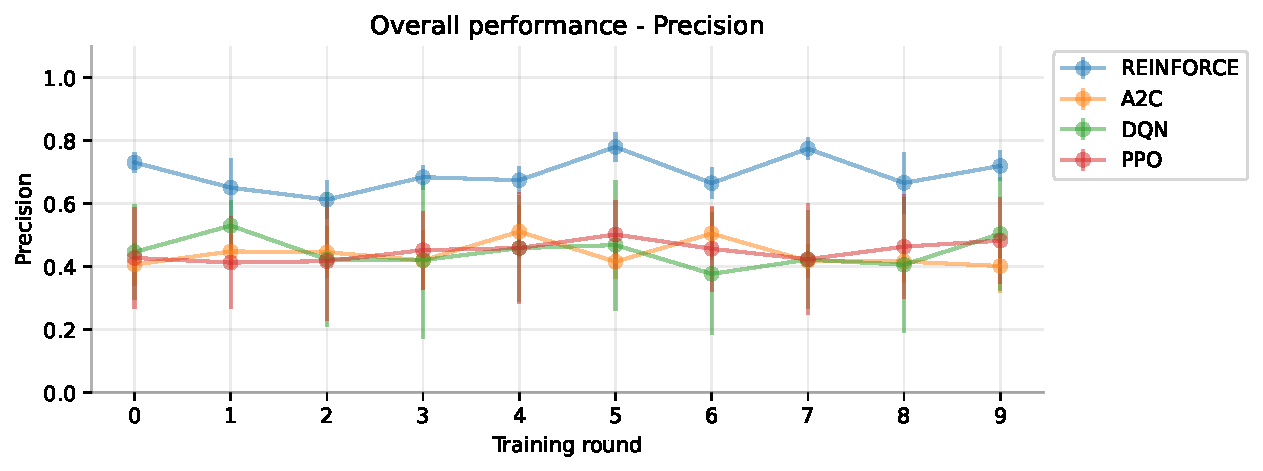
\includegraphics[width=\linewidth]{Overall_Pr.pdf}  
	\caption{Precision}
	\label{fig:tr-ovr-pr}
	\end{subfigure} \par\smallskip

	\begin{subfigure}{\textwidth}
	\centering
	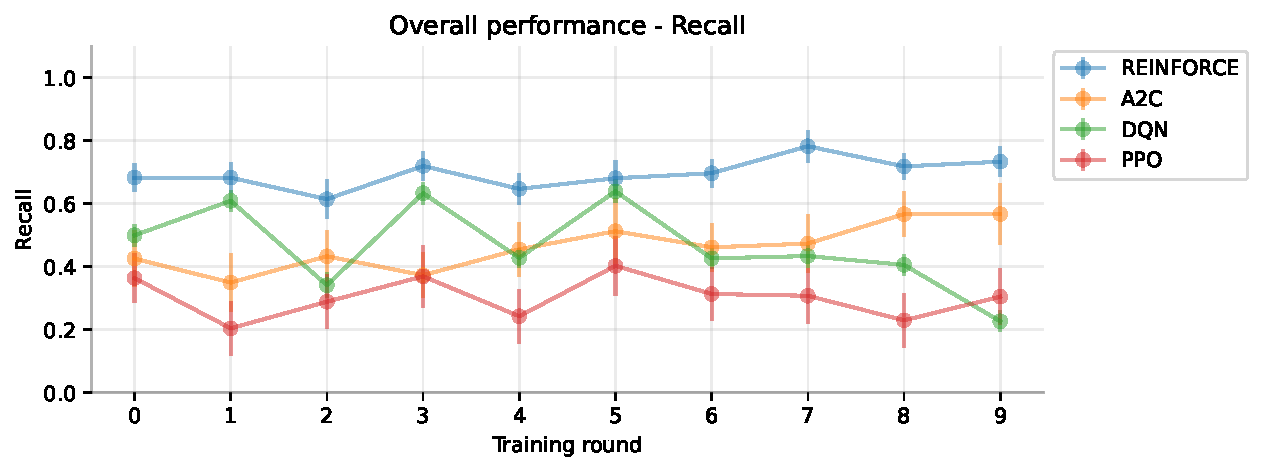
\includegraphics[width=\linewidth]{Overall_Rc.pdf}  
	\caption{Recall}
	\label{fig:tr-ovr-rc}
	\end{subfigure} \par\smallskip
	
	\begin{subfigure}{\textwidth}
		\centering
		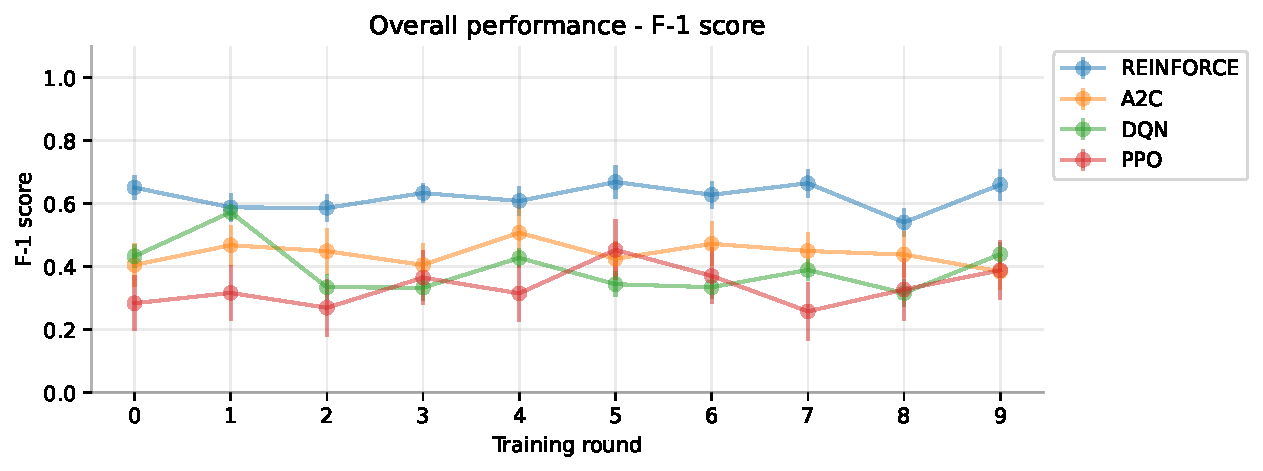
\includegraphics[width=\linewidth]{Overall_F1.pdf}  
		\caption{F1-score}
		\label{fig:tr-ovr-f1}
	\end{subfigure} \par\smallskip

	\begin{subfigure}{\textwidth}
		\centering
		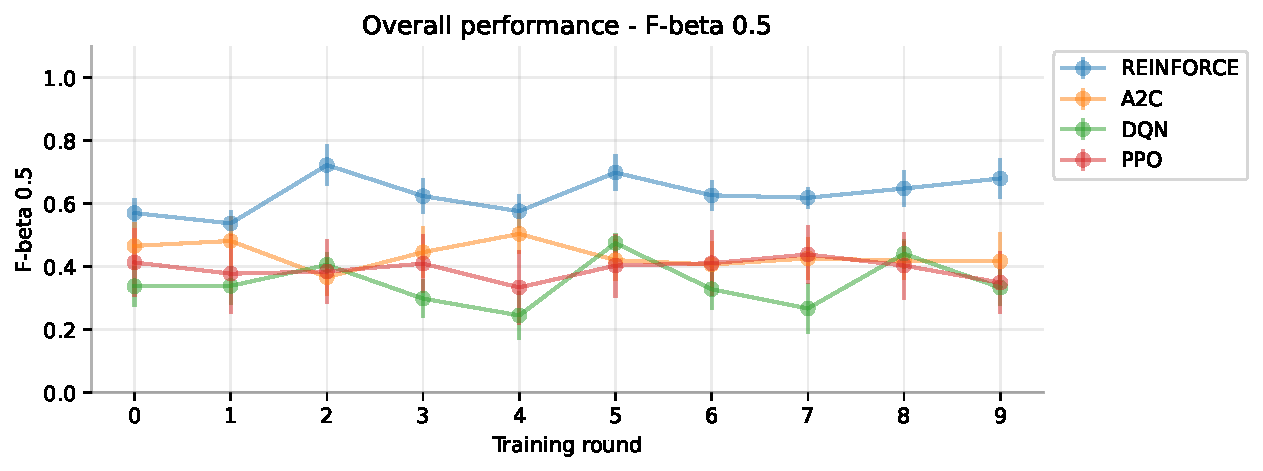
\includegraphics[width=\linewidth]{Overall_F05.pdf}  
		\caption{F-beta (0.5)}
		\label{fig:tr-ovr-f05}
	\end{subfigure}
	\caption{Overall performance -- Average over 10 models}
	\label{fig:tr-overall}
\end{figure}

\begin{figure}[ht]
	\begin{subfigure}{\textwidth}
		\centering
		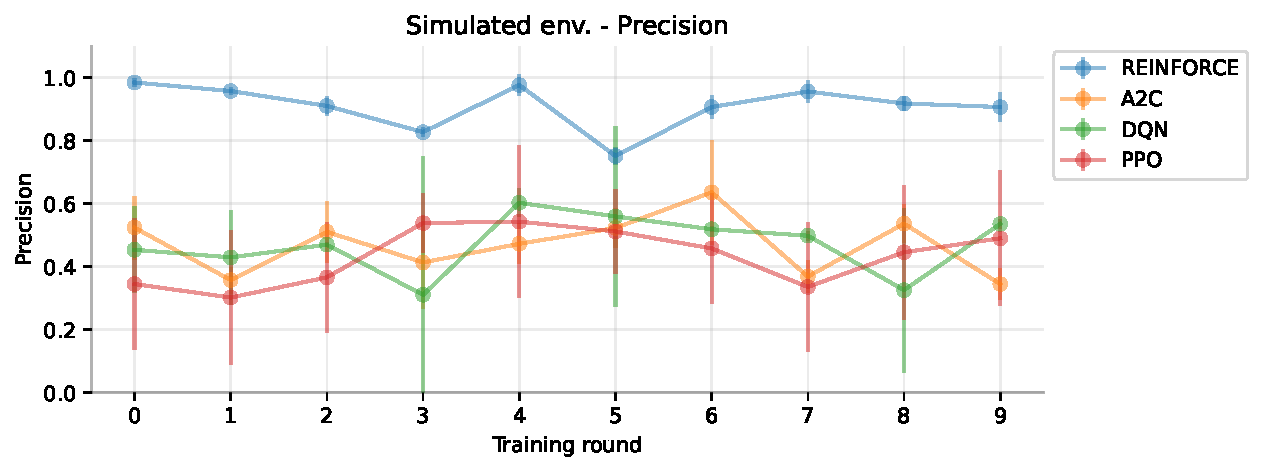
\includegraphics[width=\linewidth]{Simulated_Pr.pdf}  
		\caption{Precision}
		\label{fig:tr-sim-pr}
	\end{subfigure} \par\smallskip
	
	\begin{subfigure}{\textwidth}
		\centering
		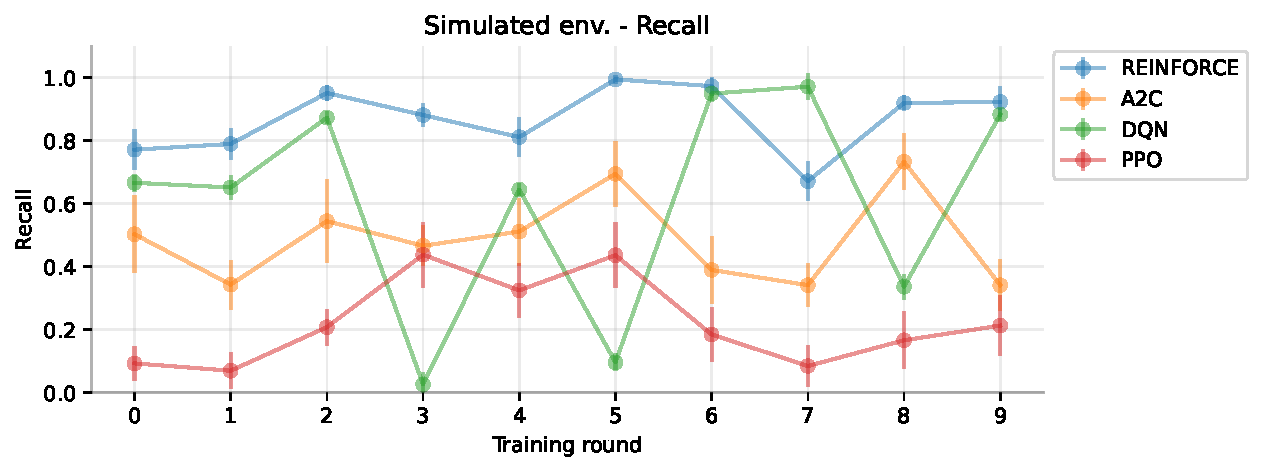
\includegraphics[width=\linewidth]{Simulated_Rc.pdf}  
		\caption{Recall}
		\label{fig:tr-sim-rc}
	\end{subfigure} \par\smallskip
	
	\begin{subfigure}{\textwidth}
		\centering
		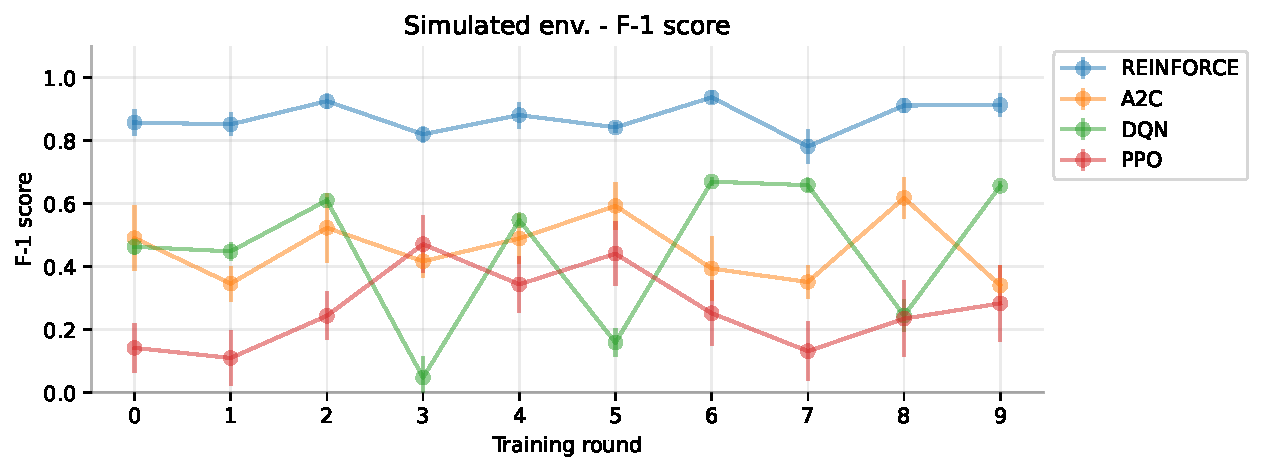
\includegraphics[width=\linewidth]{Simulated_F1.pdf}  
		\caption{F1-score}
		\label{fig:tr-sim-f1}
	\end{subfigure} \par\smallskip
	
	\begin{subfigure}{\textwidth}
		\centering
		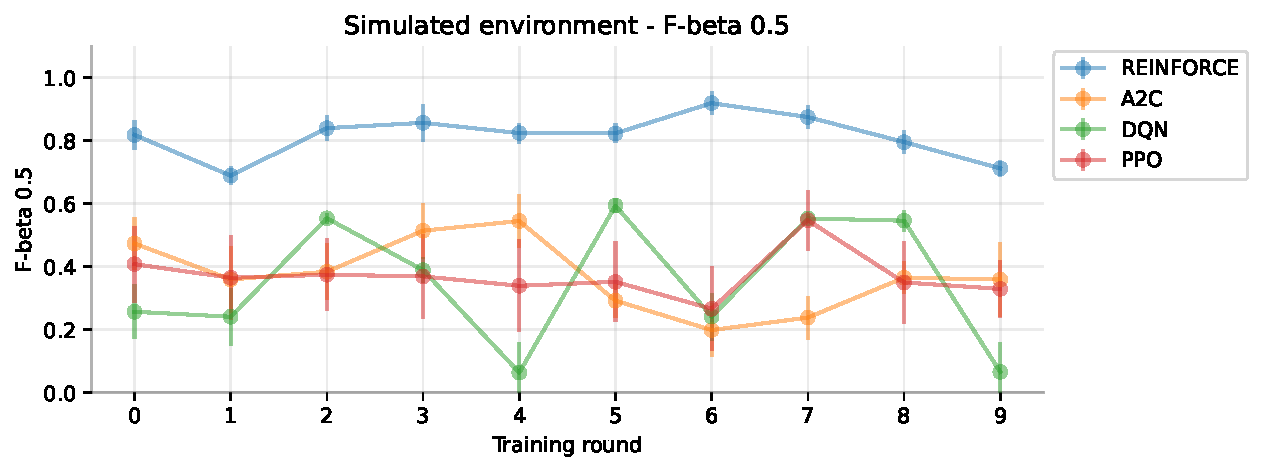
\includegraphics[width=\linewidth]{Simulated_F05.pdf}  
		\caption{F-beta (0.5)}
		\label{fig:tr-sim-f05}
	\end{subfigure}
	\caption{Simulated environment -- Average over 10 models}
	\label{fig:tr-sim-env}
\end{figure}

\begin{figure}[ht]
	\begin{subfigure}{\textwidth}
		\centering
		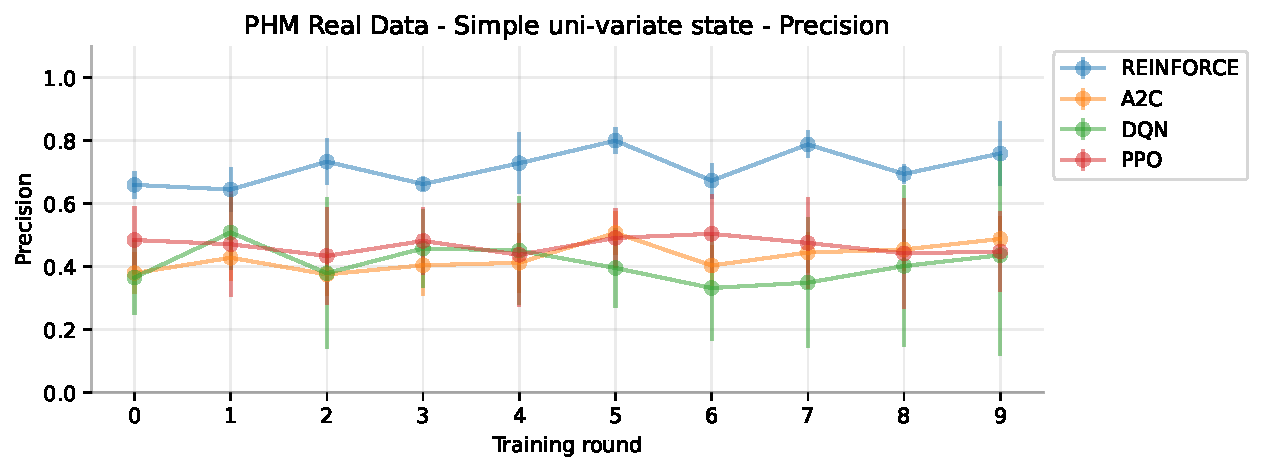
\includegraphics[width=\linewidth]{Singevariable_Pr.pdf}  
		\caption{Precision}
		\label{fig:tr-ss-pr}
	\end{subfigure} \par\smallskip
	
	\begin{subfigure}{\textwidth}
		\centering
		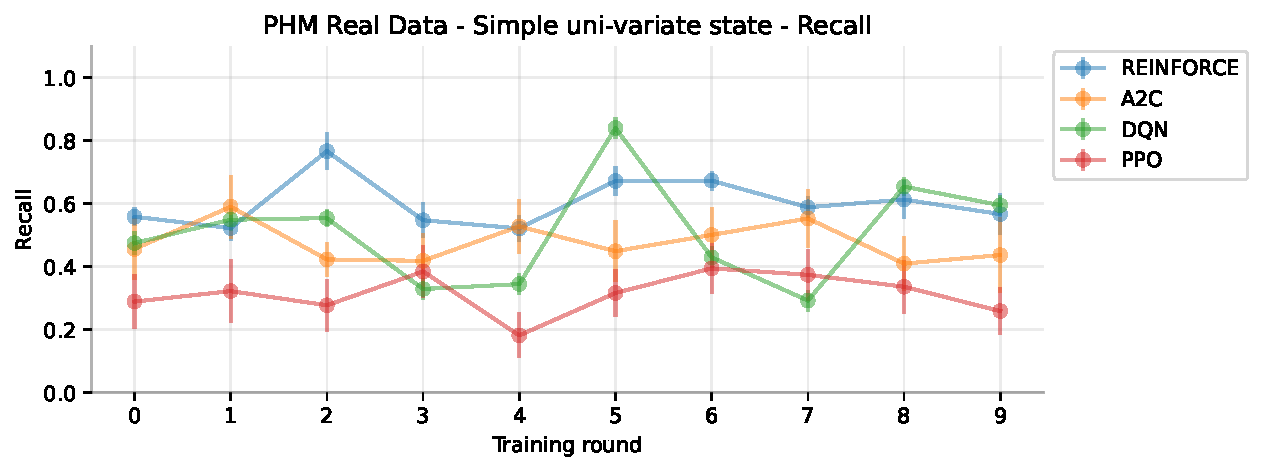
\includegraphics[width=\linewidth]{Singevariable_Rc.pdf}  
		\caption{Recall}
		\label{fig:tr-ss-rc}
	\end{subfigure} \par\smallskip
	
	\begin{subfigure}{\textwidth}
		\centering
		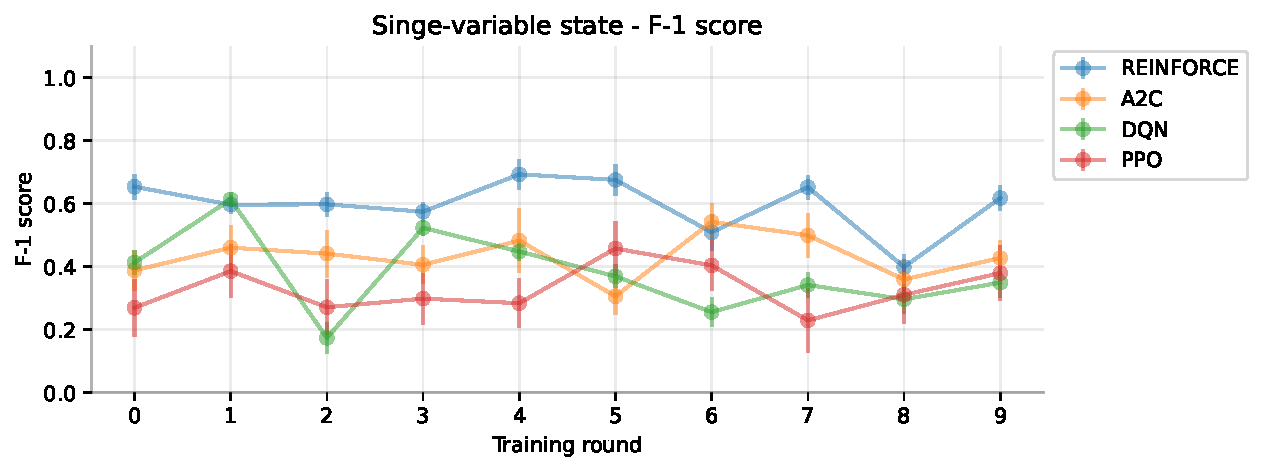
\includegraphics[width=\linewidth]{Singevariable_F1.pdf}  
		\caption{F1-score}
		\label{fig:tr-ss-f1}
	\end{subfigure} \par\smallskip
	
	\begin{subfigure}{\textwidth}
		\centering
		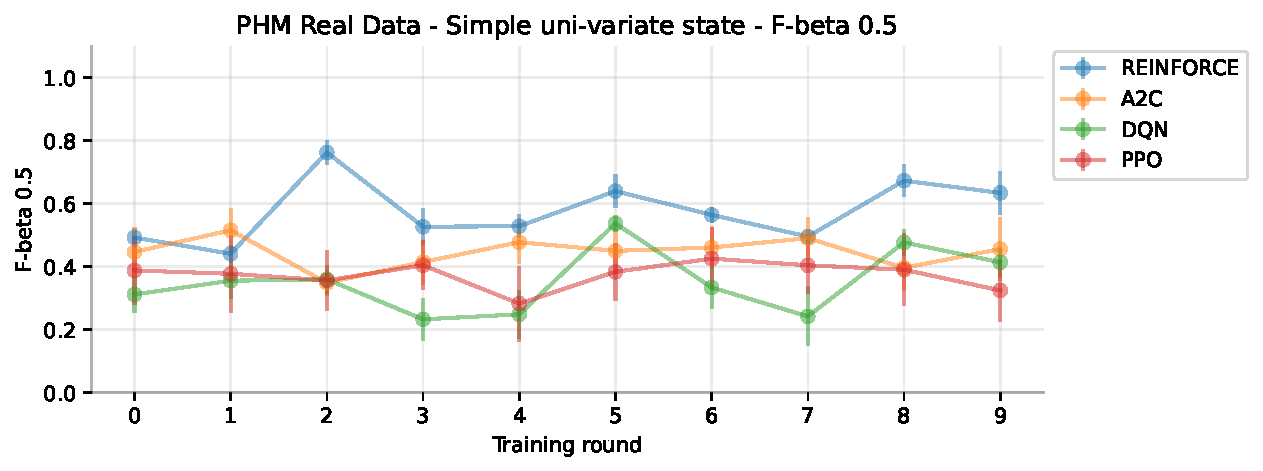
\includegraphics[width=\linewidth]{Singevariable_F05.pdf}  
		\caption{F-beta (0.5)}
		\label{fig:tr-ss-f05}
	\end{subfigure}
	\caption{Univariate state environment -- Average over 10 models}
	\label{fig:tr-ss-env}
\end{figure}

\begin{figure}[ht]
	\begin{subfigure}{\textwidth}
		\centering
		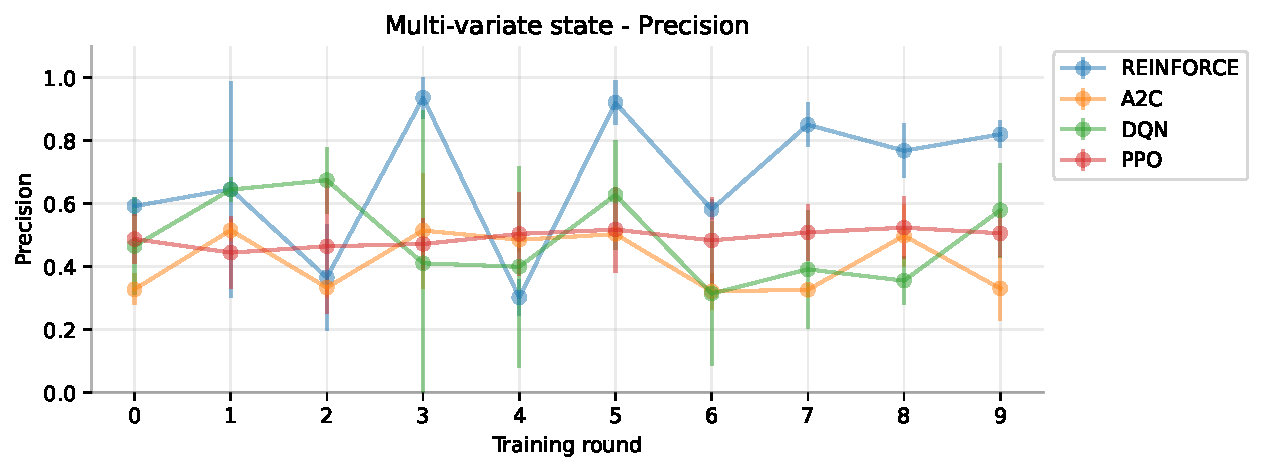
\includegraphics[width=\linewidth]{Multivariate_Pr.pdf}  
		\caption{Precision}
		\label{fig:tr-ms-pr}
	\end{subfigure} \par\smallskip
	
	\begin{subfigure}{\textwidth}
		\centering
		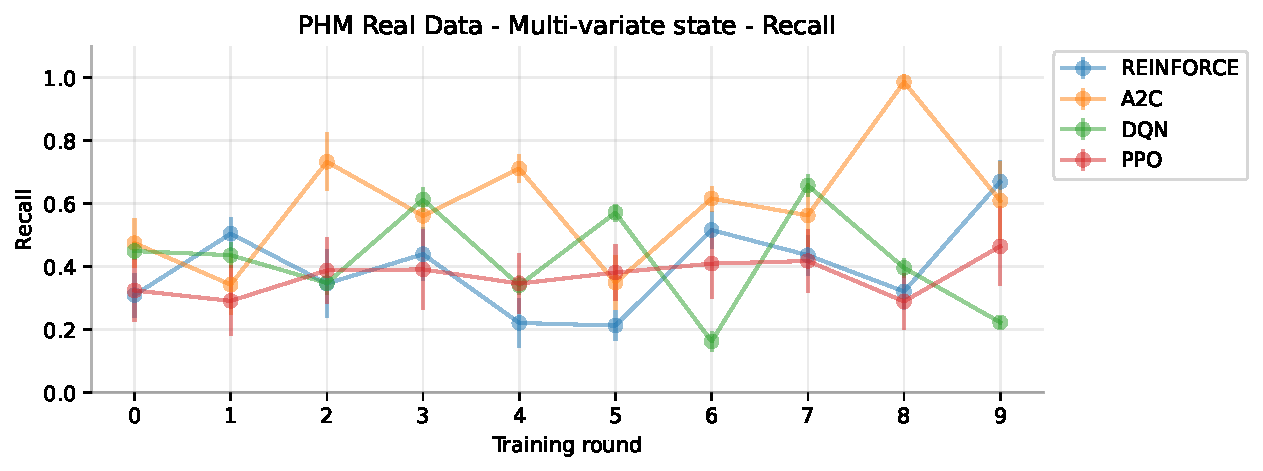
\includegraphics[width=\linewidth]{Multivariate_Rc.pdf}  
		\caption{Recall}
		\label{fig:tr-ms-rc}
	\end{subfigure} \par\smallskip
	
	\begin{subfigure}{\textwidth}
		\centering
		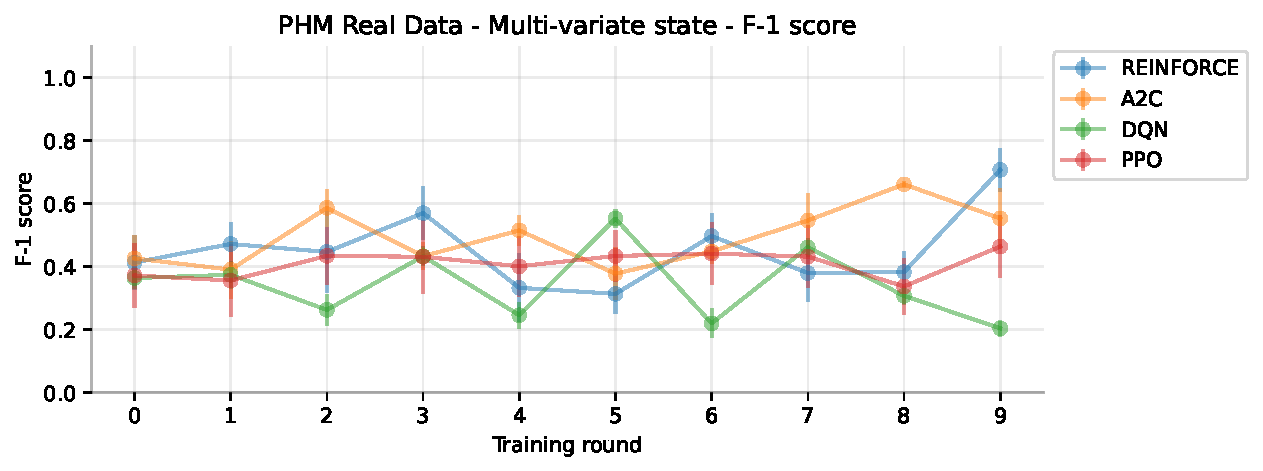
\includegraphics[width=\linewidth]{Multivariate_F1.pdf}  
		\caption{F1-score}
		\label{fig:tr-ms-f1}
	\end{subfigure} \par\smallskip
	
	\begin{subfigure}{\textwidth}
		\centering
		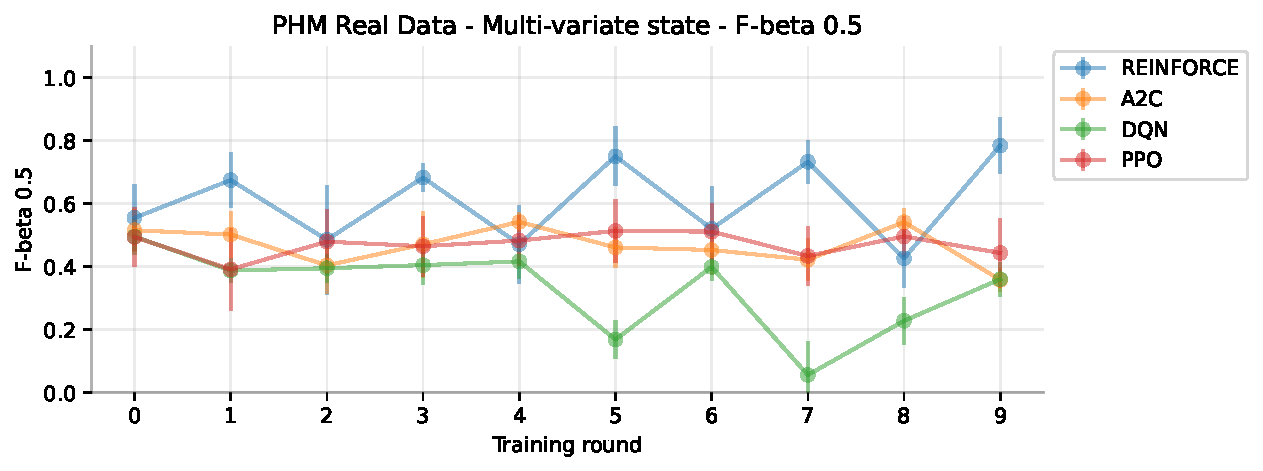
\includegraphics[width=\linewidth]{Multivariate_F05.pdf}  
		\caption{F-beta (0.5)}
		\label{fig:tr-ms-f05}
	\end{subfigure}
	\caption{Multivariate state environment -- Average over 10 models}
	\label{fig:tr-ms-env}
\end{figure}




\subsection{Super models metrics}

\newgeometry{margin=1cm} % Change margins for landscape table
\begin{landscape}\centering
	\begin{table*}
		\sffamily
		\rowspace{1.3}
		\begin{tabular}{@{}l rrrr c rrrr c rrrr c rrrr@{}} \arrayrulecolor{black!40}\toprule
			& \multicolumn{4}{c}{\textbf{REINFORCE}} & & \multicolumn{4}{c}{A2C} &
			& \multicolumn{4}{c}{DQN} & & \multicolumn{4}{c}{PPO} \\
			\cmidrule{2-5} \cmidrule{7-10} \cmidrule{12-15} \cmidrule{17-20}
			Environment &Prec. &Recall &F1 &F$_\beta$0.5 & &Prec. &Recall &F1 &F$_\beta$0.5 & &Prec. &Recall &F1 &F$_\beta$0.5 & &Prec. &Recall &F1 &F$_\beta$0.5\\ \midrule
			Simulated  - No noise &0.897 &0.960 &0.926 & 0.908 & & 0.500 &1.000 &0.667 &0.556 & &0.505 &0.980 &0.667 &0.560 & &0.669 &0.430 &0.518&0.597\\
			Simulated  - Low noise &0.960 &0.945 &0.952 & 0.957 & & 0.516 &1.000 &0.680 &0.571 & &0.500 &0.980 &0.662 &0.554 & &0.633 &0.460 &0.530&0.586\\
			Simulated  - High noise &0.922 &0.990 &0.955 & 0.935 & & 0.503 &1.000 &0.669 &0.558 & &0.504 &0.990 &0.668 &0.559 & &0.569 &0.355 &0.434&0.505\\\midrule
			
			PHM C01 SS - No noise &0.889 &0.995 &0.939 & 0.908 & & 0.586 &0.625 &0.603 &0.592 & &0.647 &0.970 &0.776 &0.693 & &0.543 &1.000 &0.703&0.597\\
			PHM C01 SS - Low noise &0.988 &0.765 &0.861 & 0.932 & & 0.499 &0.995 &0.664 &0.554 & &0.504 &0.990 &0.668 &0.559 & &0.623 &0.740 &0.675&0.643\\
			PHM C01 SS - High noise &0.850 &0.970 &0.905 & 0.871 & & 0.521 &0.680 &0.588 &0.546 & &0.505 &0.985 &0.668 &0.560 & &0.520 &0.725 &0.604&0.551\\\hdashline
			
			PHM C04 SS - No noise &0.811 &1.000 &0.895 & 0.842 & & 0.536 &0.645 &0.583 &0.554 & &0.501 &0.965 &0.660 &0.554 & &0.579 &0.895 &0.702&0.622\\
			PHM C04 SS - Low noise &0.798 &0.980 &0.879 & 0.829 & & 0.556 &0.665 &0.603 &0.573 & &0.734 &0.990 &0.843 &0.774 & &0.546 &0.660 &0.596&0.565\\
			PHM C04 SS - High noise &0.708 &0.840 &0.767 & 0.730 & & 0.521 &0.835 &0.641 &0.563 & &0.511 &0.985 &0.672 &0.565 & &0.517 &0.820 &0.633&0.558\\\hdashline
			
			PHM C06 SS - No noise &1.000 &0.895 &0.944 & 0.977 & & 0.520 &0.680 &0.587 &0.545 & &0.935 &0.975 &0.954 &0.942 & &0.587 &0.650 &0.615&0.597\\
			PHM C06 SS - Low noise &0.943 &0.795 &0.861 & 0.908 & & 0.501 &1.000 &0.668 &0.557 & &0.961 &0.725 &0.826 &0.901 & &0.552 &0.370 &0.438&0.497\\
			PHM C06 SS - High noise &0.821 &0.845 &0.831 & 0.825 & & 0.540 &0.755 &0.628 &0.572 & &0.980 &0.960 &0.969 &0.976 & &0.521 &0.615 &0.564&0.537\\\midrule
			
			PHM C01 MS - No noise &0.827 &0.995 &0.903 & 0.856 & & 0.500 &1.000 &0.667 &0.556 & &0.505 &0.985 &0.668 &0.560 & &0.512 &0.595 &0.549&0.526\\
			PHM C04 MS - No noise &0.910 &0.425 &0.577 & 0.738 & & 0.500 &1.000 &0.667 &0.556 & &0.501 &0.975 &0.662 &0.555 & &0.501 &0.635 &0.558&0.522\\
			PHM C06 MS - No noise &0.934 &0.865 &0.896 & 0.918 & & 0.500 &1.000 &0.667 &0.556 & &0.969 &0.600 &0.741 &0.863 & &0.497 &0.690 &0.577&0.526\\			
			\bottomrule
		\end{tabular}
		\caption{Super Models: Best models selected over 10 rounds of training.}
		\label{tbl:SuperModels}
	\end{table*}
\end{landscape}
\restoregeometry % Restore margins after landscape table


\subsection{Hypothesis testing}

Notes: \\
- Definition of 1 data point\\
- Single training round (5th of the 10 rounds)\\
- Single dataset:  PHM C01\\
- Single env:  Simple univariate state\\
- Single noise setting:  HBD = high\\
- File has 40 rows = 4 algos x 10 test rounds\\
- 10 test rounds of 40 random sampled points\\
- 1 point = 1 row = 1 classification test with 40 samples\\
- E.g. Dasic = 10 training rounds x 10 test rounds x 3 noise settings = 300 sample points\\
- E.g. PHM SS = 3 datasets x 10 training rounds x 10 test rounds x 3 noise settings = 900 sample points\\
- Technically Dasic = 300 points for metrics = 300 * 40 sampled data points of wear data = 12000\\



\begin{equation}
	\left.\begin{aligned}
		H_0 & : \mu_{RF} - \mu_{AA} = 0,\;\; \\
		H_a & : \mu_{RF} - \mu_{AA} > 0, \;\;
	\end{aligned}
	\right\}
	\qquad \forall \;\; \text{$AA \in[A2C, DQN, PPO]$}
\end{equation}

\begin{table*}[hbt!]\centering
	\sffamily
	\rowspace{1.3}
	\begin{tabular}{@{}l c rrr c l rrr @{}}
		\arrayrulecolor{black!40}\toprule
		
		&& \multicolumn{3}{c}{\textbf{p Value}} & \phantom{i} & & \multicolumn{3}{c}{\textbf{t Statistic}} \\
		\cmidrule{3-5} \cmidrule{8-10} 
		
		Metric && \small {RF $\underset{H_0}{\overset{H_a}{\geqq}}$ A2C} &\small {RF $\underset{H_0}{\overset{H_a}{\geqq}}$DQN} &\small {RF $\underset{H_0}{\overset{H_a}{\geqq}}$PPO} & & & \small {RF $\underset{H_0}{\overset{H_a}{\geqq}}$ A2C} &\small {RF $\underset{H_0}{\overset{H_a}{\geqq}}$DQN} &\small {RF $\underset{H_0}{\overset{H_a}{\geqq}}$PPO} \\ \midrule 
		\multicolumn{10}{@{}l}{\textbf{Overall} (1500 samples)} \\[6pt]
		Precision & &4.31E-126 &2.17E-109 &2.81E-106 & & &25.071 &23.170 &22.804\\
		Recall & &4.20E-35 &3.37E-16 &4.36E-150 & & &12.522 &8.206 &27.650\\
		F1 score & &1.99E-64 &1.46E-88 &5.29E-155 & & &17.364 &20.634 &28.160\\[6pt]\midrule
		
		\multicolumn{10}{@{}l}{\textbf{Simulated environment} (300 samples)}\\[6pt]
		Precision & &3.20E-98 &1.69E-63 &2.65E-81 & & &25.611 &19.032 &22.427\\
		Recall & &8.12E-104 &2.56E-41 &1.57E-264 & & &26.665 &14.558 &62.541\\
		F1 score & &9.60E-134 &8.56E-99 &2.96E-242 & & &32.402 &25.719 &56.575\\[6pt] \midrule
		
		\multicolumn{10}{@{}l}{\textbf{PHM Real data - Simple univariate state} (900 samples)} \\[6pt]
		Precision & &2.27E-32 &7.29E-31 &9.95E-31 & & &12.082 &11.770 &11.742\\
		Recall & &1.27E-16 &1.55E-06 &8.19E-71 & & &8.357 &4.821 &18.607\\
		F1 score & &1.94E-19 &4.67E-34 &2.19E-67 & & &9.121 &12.423 &18.098\\ [6pt]\midrule
		
		\multicolumn{10}{@{}l}{\textbf{PHM Real data - Complex multivariate state} (300 samples)}\\[6pt]
		Precision & &1.64E-60 &3.34E-54 &7.88E-59 & & &18.451 &17.207 &18.122\\
		Recall & &2.69E-10 &2.69E-02 &9.68E-01 & & &-6.425 &-2.219 &-0.041\\
		F1 score & &7.27E-01 &1.44E-08 &1.35E-03 & & &0.349 &5.748 &3.220\\
		\bottomrule
	\end{tabular}
	\caption{One-tail t-test - Ho: No difference in metrics. Ha: REINFORCE metric > Advanced algorithm metric}
	\label{tbl:ttest}
\end{table*}



\subsection{Training times}
\begin{figure}[ht]
	\centering
	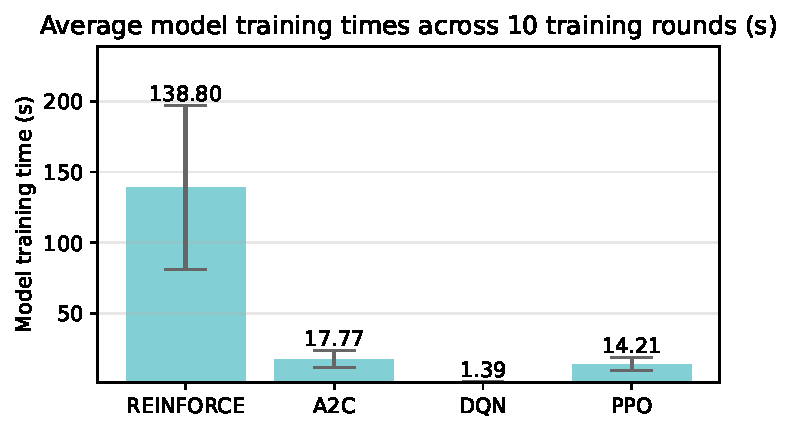
\includegraphics[width=\linewidth]{Model_training_time.pdf}  
	\caption{Training time. Across 10 rounds and all environment variants.}
	\label{fig:tr-time}
\end{figure}






\section{Discussion}\label{sec:Discussion}

\textcolor{red}{**\textbf{DISCUSSION}** It must be noted that the classification metrics we used to evaluate, assume that the human prevent maintenance policy is ideal and suggested based on experience. In practice this might not always be the case. The RL agent is trained to replace the tool optimally i.e. maximize use before reaching the threshold use, and replace only when necessary so as to maintain lowest possible cost of replacement. In our dataset we assume the threshold to be ideally set and base the ``human'' action against that, rather than a real human action, which incidentally is not available for the PHM dataset anyway.}

\begin{itemize}
	\item R1 = +1 
	\item R2 = -1
	\item R3 = -100 => higher neg. Improve recall. Lower neg. Improve precision. 
	\item Hyper-parameters for Precision or Recall control: 
	\item Precision => low FP => False replacement-action reduced. \textcolor{red}{***} Unnecessary tool replacement reduced. Tool life maximized, down time minimized, production disruption minimized. 
	\item - Recall => low FN => False declaration of normal operation reduced. Reduce missed replacements. Tool replacements increased. \textcolor{red}{***} Product quality not compromised. 
	\item \textbf{LOOK AHEAD PARAM}: 
	\item  It must be noted that the classification metrics we used to evaluate, assume that the human prevent mainteance policy is ideal. Which in practice might not be the case. The RL is trained to replace the tool optimally i.e. maximize use and replace only when necessary so as to maintain lowest possible cost of replacement.
\end{itemize}

- Transition function \citep{graesser2019}: pg333 "Transition function  - also known as model. can be learnt or programmed programmable rules are common and lead to increasing complexity. \textcolor{red}{***} We use a hybrid model - partly learnt and partly programmed": \textbf{Noise and breakdown}\\


\cite{duan2016benchmarking} the environment.\textcolor{red}{*OBSERVATION**}REINFORCE: Despite its simplicity, REINFORCE is an
effective algorithm in optimizing deep neural network policies
in most basic and locomotion tasks. Even for high-
DOF tasks like Ant, REINFORCE can achieve competitive
results. However we observe that REINFORCE sometimes
suffers from premature convergence to local optima
as noted by Peters  Schaal (2008), which explains the performance
gaps between REINFORCE and TNPG on tasks
such as Walker (Figure 3(a)). By visualizing the final policies,
we can see that REINFORCE results in policies that
tend to jump forward and fall over to maximize short-term
return instead of acquiring a stable walking gait to maximize
long-term return. In Figure 3(b), we can observe
that even with a small learning rate, steps taken by REINFORCE
can sometimes result in large changes to policy
distribution, which may explain the fast convergence to local
optima.


\subsection{Precision or Recall?}
- Precision => low FP => False replacement-action reduced. \textcolor{red}{***} Unnecessary tool replacement reduced. Tool life maximized, down time minimized, production disruption minimized \\
- Recall => low FN => False declaration of normal operation reduced. Reduce missed replacements. Tool replacements increased. \textcolor{red}{***} Product quality not compromised. 


limitiongs of the slecting model for evaluation

\cite{SB3-paper} -- quote from paper - intro section -- "A major challenge is that small implementation details can have a substantial effect on performance often greater than the difference between algorithms (Engstrom et al., 2020). It is particularly important that  implementations used as experimental baselines are reliable; otherwise, novel algorithms compared to weak baselines lead to inated estimates of performance improvements"

DPO paper - Rafael Rafailov May-2023 --- Direct Preference Optimization: Your Language Model is Secretly a Reward Model 

5.2 Instability of Actor-Critic Algorithms
We can also use our framework to diagnose instabilities with standard actor-critic algorithms used
for the RLHF, such as PPO. We follow the RLHF pipeline and focus on the RL fine-tuning step
outlined in Section 3. We can draw connections to the control as inference framework [18] for the
constrained RL problem outlined in 3. We assume a parameterized model and minimize
This is the same objective optimized in prior works [45, 35, 1, 23] using the DPO-equivalent reward
for the reward class of In this setting, we can interpret the normalization term in 
as the soft value function of the reference policy . While this term does not affect the optimal
solution, without it, the policy gradient of the objective could have high variance, making learning
unstable. We can accommodate for the normalization term using a learned value function, but that
can also be difficult to optimize. Alternatively, prior works have normalized rewards using a human
completion baseline, essentially a single sample Monte-Carlo estimate of the normalizing term. In
contrast the DPO reparameterization yields a reward function that does not require any baselines.

\section{Conclusion}\label{sec:Conclusion}


%% References
\bibliographystyle{plainnat}
\bibliography{ES_bibliography}
\end{document}
